This chapter provides more background information on the Merlion 
water quality model and discusses a few of the more advanced topics 
for the sensor placement problem. In addition, a few case study applications 
using the different WST subcommands are provided.

\section{Merlion Water Quality Model}\label{appendixMerlion} 
The Merlion water quality modeling framework is provided with WST to enable
fast multi-scenario simulations and solution of optimization problems that require
an embedded water quality model (e.g., booster placement with \code{booster\_mip}, source identification MIP formulation). 
In this section, the model equations and the calculations performed inside WST 
in order to generate a linear system of equations to describe the water
quality in a network are briefly described. The equations and the discretization process described in 
this section do not require any additional work from the user (except for selecting the merlion 
option in the configuration file). More details about the Merlion modeling framework is provided in \citep{Merlion12}.   
      
The model formulation ensures mass balances
at all junctions, pipes and tanks. The following mass balance equations
describe the transport of a species inside the network. For simplicity,
complete instantaneous mixing is assumed for the tanks, and plug flow
is assumed for the pipes.

\bigskip{}

\begin{equation}
c_{n}(t)=\dfrac{\sum_{i\in\Gamma_{n}^{O}(t)}Q_{i}(t)\hat{c}_{i}^{O}(t)-\sum_{i\in\Gamma_{n}^{I}(t)}Q_{i}(t)\hat{c}_{i}^{I}(t)+m_{n}(t)}{\sum_{i\in\Gamma_{n}^{O}(t)}Q_{i}(t)-\sum_{i\in\Gamma_{n}^{I}(t)}Q_{i}(t)+Q_{n}^{ext}(t)},\;\;\forall\;
n\in\mathbf{J} \label{eq:junctionbalance}
\end{equation}

\medskip{}

\begin{multline}
V_{n}(t)\dfrac{dc_{n}(t)}{dt}=\sum_{i\in\Gamma_{n}^{O}(t)}Q_{i}(t)\hat{c}_{i}^{O}(t)-\sum_{i\in\Gamma_{n}^{I}(t)}Q_{i}(t)\hat{c}_{i}^{I}(t)+m_{n}(t)\\
-\left[\sum_{i\in\Gamma_{n}^{O}(t)}Q_{i}(t)-\sum_{i\in\Gamma_{n}^{I}(t)}Q_{i}(t)+Q_{n}^{\mathrm{ext}}(t)\right]c_{n}(t),\;\;\forall\; n\in\mathbf{ST}\label{eq:tankbalance}
\end{multline}

\bigskip{}

\begin{equation}
\dfrac{\partial\hat{c}_{i}(x,t)}{dt}+u_{i}(t)\dfrac{\partial\hat{c}_{i}(x,t)}{dx}=0,\forall i\in\mathbf{P}\label{eq:pipebalance}
\end{equation}

where $c_{n}$ and $m_{n}$ denotes the concentration and mass injected at a node,
respectively. The variable $\hat{c}_{i}$ is the concentration inside pipe $i$ 
and $V_{n}$ is the volume of water inside tank $n$.
The variable $\mathbf{{J}}$ is a set of all junctions, $\mathbf{{ST}}$
is a set of all storage tanks and $\mathbf{{P}}$ is a set of all
pipes. The variable $Q$ denotes volumetric flow rates that are pre-calculated using
EPANET 2.00.12 and are assumed to be constant over each hydraulic time step.
The flow rate of a known external source entering a node is also pre-calculated
and is denoted by $Q_{i}^{\mathrm{ext}}$. The variable $\Gamma_{n}^{O}$ represents the
set of all pipes with flow going away from node $n$. Similarly,
$\Gamma_{n}^{I}$ represents the set of all pipes with flow coming
into node $n$. 

Equation~\ref{eq:junctionbalance} represents a set of algebraic equations
dependent on time alone and Equation~\ref{eq:tankbalance} represents
a set of ordinary differential equations (ODEs) also dependent on time alone. Therefore, these two equations
can be discretized in time. However, discretizing Equation~\ref{eq:pipebalance},
which are partial differential equations (PDEs), in both time and space would lead to a prohibitively
large model. Instead, these pipe balance PDEs are replaced using an origin-tracking
algorithm. This algorithm is based on the Lagrangian method; however,
instead of tracking concentration values as packets of water moving
through the network, the origin-tracking algorithm tracks the originating
node and time step of each packet as it enters a pipe (see Figure \ref{fig:origin_figure}). 
Once the water packet exits the pipe, equations are written relating
the concentration of the pipe inlet and outlet to the concentration
of connected nodes based on time delay. These time delay expressions
are formulated for each pipe independently. Therefore, the algorithm
scales favorably for a large water distribution system having a linear
computational cost as the size of the network increases. 

\begin{figure}[!h]
\begin{center}
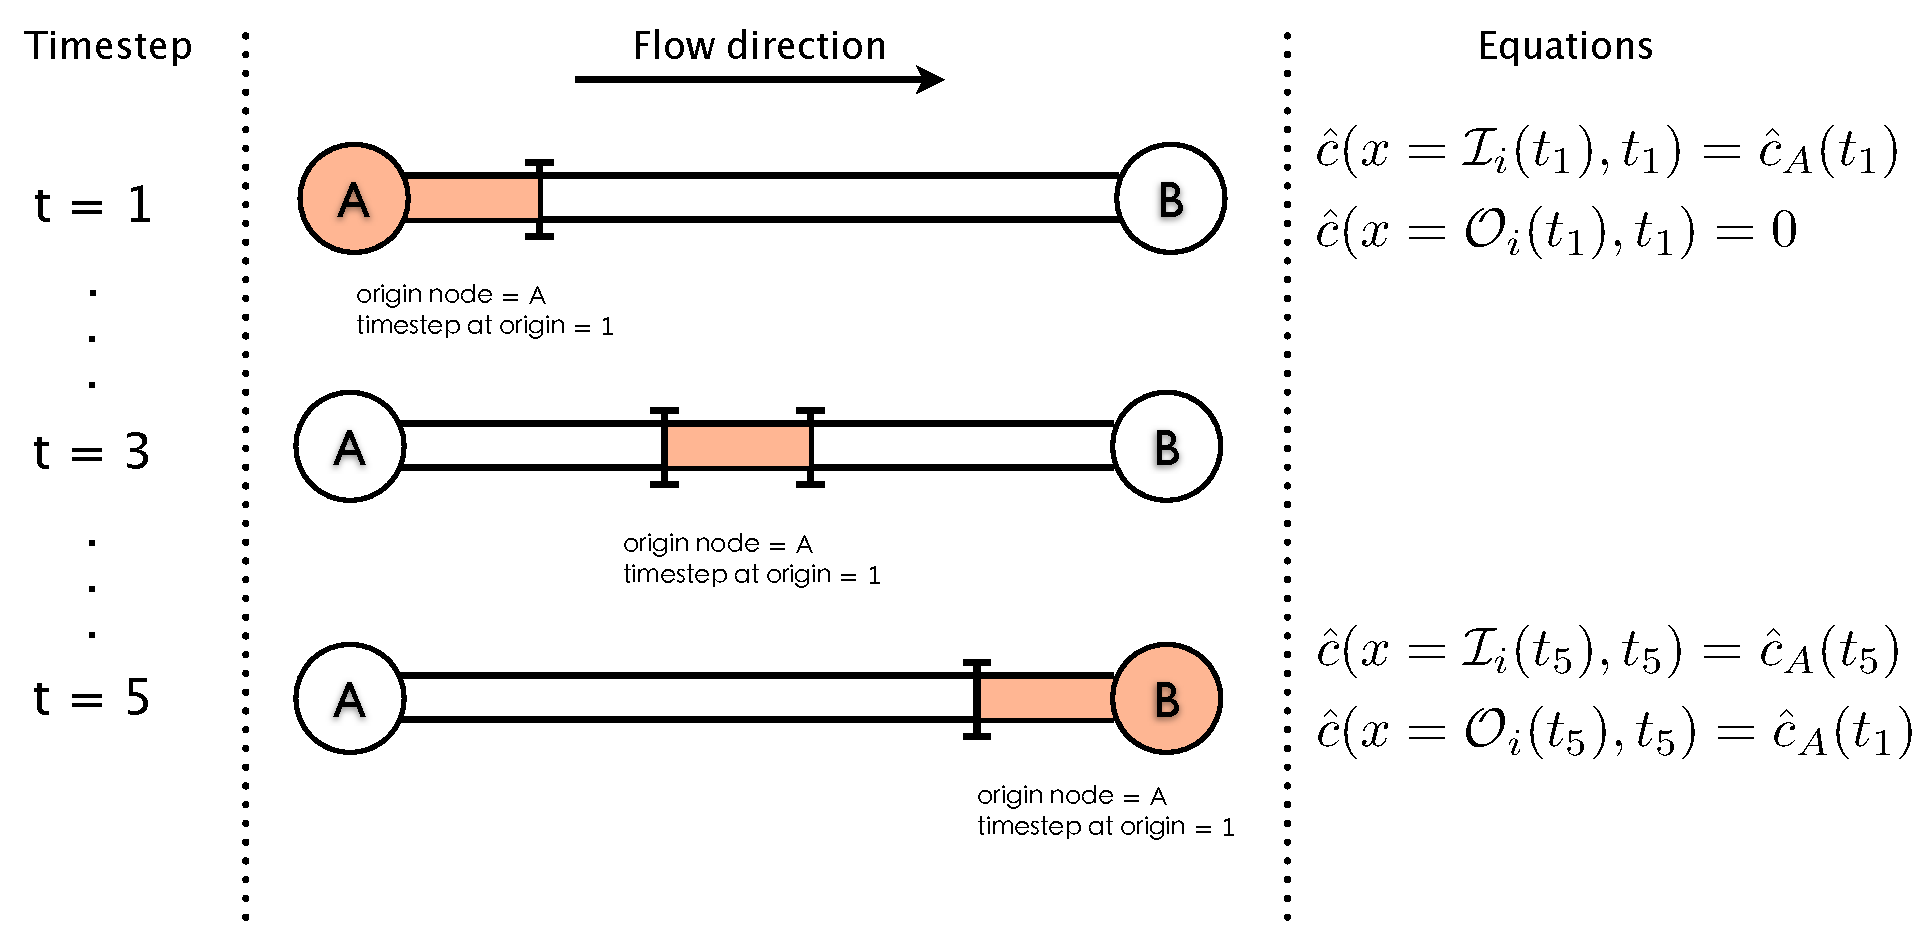
\includegraphics[scale=0.38]{graphics/origin_figure.pdf}\caption{Illustration of the origin tracking algorithm.}
\label{fig:origin_figure}
\end{center}
\end{figure}


By calculating time delay expressions, a very large but sparse linear
system of equations is generated that relates 
%The time delay expressions are included in the mass balance equations
%to form a large but very sparse linear system relating 
input injections ($m$)
from all nodes and time steps to output concentrations ($c$) from
all nodes and time steps.

\begin{equation}
Gc=Dm\label{eq:Merlion_Model}
\end{equation}


Unlike black box simulations, this linear model can be extended and
embedded inside other numerical applications. For example, the water quality model can be
embedded inside a mathematical programming formulation for applications
like booster placement, source inversion and optimal grab sampling. 

After formulating the linear system, performing a tracing simulation
is straightforward. First, an injection profile ($m$) is specified.
Then, the system is factorized and finally backsolved for the network
concentration profile $c$. This process is fast, and even more efficient
when simulating a large ensemble of tracing simulations. In this case,
the system is factorized once, and a backsolve is performed for each
simulation. To get additional speedup, a tailored solver is also provided
that takes advantage of the structure of the linear system by permuting
matrix $G$ into lower triangular, which removes the need for any
factorization. The tailored solver also utilizes the Basic Linear
Algebra Sub-routines (BLAS) library to perform multiple backsolves
(corresponding to multiple injection scenarios) more efficiently. 
For additional information about Merlion, refer to \citet{Merlion12}. 
%\mathbf{NOTE: Merlion currently only supports time based controls. 
%All EPANET networks INP files provided with WST have been modified by 
%converting all conditional controls to time based controls. This was 
%done by running the hydraulics and finding the first time at which a 
%conditional control was trigger and then enforcing a time based control 
%at the closest earlier hydraulic time step.} 

\newpage

\section{Average-case Sensor Placement}\label{chap:pmedian} 

The \code{sp} subcommmand can design a sensor network for contamination
warning systems (CWSs) using a variety of different optimization
formulations. The most widely studied sensor placement formulation
for CWS design is to minimize the expected impact of an ensemble
of contamination incidents given a sensor budget. This formulation
has also become the standard formulation for \code{sp}, because it
can be effectively used to select sensor placements in large water
distribution networks. This chapter provides a variety of examples
that illustrate the application of the \code{sp} subcommand for this optimization formulation.
Sensor placement formulation and examples illustrating common use of \code{sp} are included in Chapter~\ref{chap:sp}.

\subsection{Computing a Bound on the Best Sensor Placement Value}\label{solvers_solvers2a}

A mixed-integer program (MIP) solver like GLPK provide upper and lower bounds on the value
of the final solution. For large water distribution systems, it
might be prohibitively expensive to perform optimization with a MIP
solver. However, computing a lower bound with these solvers might
be practical even for large water distribution systems.

The configuration file shown in Figure \ref{fig:sp_bound}
defines a sensor placement problem with the compute bound option set to true in the 
problem block. This option indicates that the goal for the optimizer is to compute a lower bound 
on the globally optimal solution, rather than finding a sensor placement. 
All other options are those previously defined in example 3 of the Sensor 
Placement Examples (See Section~\ref{sp_example}).

\begin{figure}[h]
  \unknownInputListing{examples/sp/sp_bound.yml}{}{1}{28}
  \caption{The \code{sp} configuration file using the GLPK solver to compute a lower bound.}
  \label{fig:sp_bound}
\end{figure}

The YAML output file in Figure \ref{fig:sp_bound_output} contains the lower bound value. 
This is the same value as the solution generated by the GRASP heuristic in 
example 3 of the Sensor Placement Examples (See Section~\ref{sp_example}). 
In this manner, a MIP solver can be used to evaluate whether a heuristic 
sensor placement is near-optimal.

\begin{figure}[h]
  \unknownInputListing{examples/sp/sp_bound_output.yml}{}{1}{14}
  \caption{The \code{sp} YAML file with the lower bound from the GLPK solver.}
  \label{fig:sp_bound_output}
\end{figure}

The Lagrangian heuristic leverages the structure of the eSP model (Equations~\ref{eqn:eSP}) to
guide its search. Specifically, this heuristic computes the optimal values for the 
integer relaxation of eSP and then applies a randomized rounding technique.
As a consequence, this heuristic can also be used to compute bounds on the value of 
sensor placement in a manner that is similar to a MIP solver.
The configuration file in Figure 
\ref{fig:sp_bound_lag} uses the Lagrangian solver to determine the sensor placement 
for example 3 of the Sensor Placement Examples (See Section~\ref{sp_example}). 

\begin{figure}[h]
  \unknownInputListing{examples/sp/sp_bound_lag.yml}{}{1}{28}
  \caption{The \code{sp} configuration file using the Lagrangian solver.}
  \label{fig:sp_bound_lag}
\end{figure}

The YAML output file in Figure \ref{fig:sp_bound_lag_yaml} shows
the results of sensor placement using the Lagrangian solver for
example 3 of the Sensor Placement Examples (See Section~\ref{sp_example}).
It contains the sensor locations (EPANET IDs), the objective value
(the impact metric value), the lower bound on this objective as
well as the upper bound, which is the same as the objective value.
The sensor locations identified are nodes 139,
161, 191 and 208. The mean extent of contamination (EC) impact for
this design is approximately 9889 pipe feet contaminated. The lower
bound is approximately 9819 pipe feet contaminated, which is greater than the
bound computed by GLPK. This illustrates the fact that the bounds computed
by the Lagrangian solver are weaker than those computed by a MIP solver.

\begin{figure}[h]
  \unknownInputListing{examples/sp/sp_bound_lag_output.yml}{}{1}{14}
  \caption{The \code{sp} YAML file with the lower bound from the Lagrangian solver.}
  \label{fig:sp_bound_lag_yaml}
\end{figure}

As with MIP solvers, the Lagrangian solver can also be used to simply compute this lower bound.  
The configuration file in Figure \ref{fig:sp_bound_only_lag} shows an example of using the 
compute bound option in the problem block with the Lagrangian solver.

\begin{figure}[h]
  \unknownInputListing{examples/sp/sp_bound_only_lag.yml}{}{1}{29}
  \caption{The \code{sp} configuration file using the Lagrangian solver and the compute bound option.}
  \label{fig:sp_bound_only_lag}
\end{figure}

\subsection{Managing Sensor Placement Locations}\label{solvers_solvers2c}

By default, the \code{sp} subcommand assumes that all node locations in
a water distribution network are feasible sensor locations. 
In practice, sensors cannot be practically installed in many locations without
significant cost and inconvenience. The location block in the 
configuration file is used to specify options for declaring feasible and infeasible
node locations in the network. Additionally, the location block
can be used to declare node locations as fixed, where a sensor must be
placed, and unfixed, where a sensor cannot be located.

A location block consists of a list of declarations that are
interpreted in their order within the configuration file. Each
declaration consists of a dictionary with a single key, whose value
is either a string or list of EPANET node IDs. For example, the following location
block declares a list of infeasible node locations:
\unknownInputListing{examples/sp/fixed1.yml}{block}{22}{28}

The impact of infeasible sensor locations on the results
for example 1 of the Sensor Placement Examples (See
Section~\ref{sp_example}) is shown in following example. The solution from this example placed
sensors at nodes 113, 121, 141, 163 and 209 and the mean extent of
contamination (EC) for this sensor design was 8655. If these nodes
were listed as infeasible sensor locations (as shown in the location
block above) in the configuration file, the new sensor locations
are nodes 111, 119, 169, 207 and 237. The mean EC for this new
solution is 8932 which is worse than the initial design; this
reflects the fact that a sensor design that can use any location
will be better than a sensor design that can use a limited set of
locations.


\subsection{Limited-\/Memory Sensor Placement Techniques}\label{solvers_solvers5}

Controlling the memory used by optimizers is a critical issue when
solving large sensor placement formulations. This is a particular
challenge for MIP methods, but both the GRASP and Lagrangian
heuristics can exceed a workstation's memory when solving very large
problems. The \code{sp} subcommand supports a variety of mechanisms
that reduce the problem representation size while preserving the
structure of the sensor placement problem. These techniques include:
scenario aggregation and filtering, feasible locations, witness
aggregation, skeletonization and explicit memory management.

\paragraph{Scenario Aggregation:}
Scenario aggregation compresses the data in an impact file while
preserving its fundamental structure. This strategy is effective
when optimizing for mean performance objectives. Scenario aggregation
is performed with the \code{scenarioAggr} command, which is described
in Section~\ref{scenarioAggrExecutable}.

\paragraph{Filtering Impacts:}
Filtering impacts can also reduce memory requirements for sensor
placement by reducing the size of the impact files. Filtering can
limit the sensor placement formulation to only consider contamination
incidents that are sufficiently bad in the worst-\/case. Filtering
is performed with the \code{filter\_\-impacts} executable, which
is described in Section~\ref{filter_impactsExecutable}

\paragraph{Feasible Locations:}
Limiting the feasible locations is another strategy to reduce memory
requirements. The size of the sensor placement formulation
decreases as the number of feasible locations decreases. The
location block option described in Section~\ref{solvers_solvers2c}
can be used to specify the set of feasible locations.

\paragraph{Witness Aggregation:}
Witness aggregation limits the size of the sensor placement formulation
by aggregating the decision variables that witness a contamination
incident. By default, variables that witness contamination incidents
with the same impact are aggregated, and this typically reduces the
MIP constraint matrix by a significant amount. Further reductions
perform more aggressive aggregations that create an approximate
sensor placement formulation.

Witness aggregation is specified using an \code{aggregate} block
in the \code{sp} configuration file. A named aggregation block
specifies the type of aggregation, the aggregation limit value and
the associated impact data. For example:\newline
\begin{minipage}{\textwidth}
\begin{unknownListing}
aggregate: 
- name: agg1
  type: PERCENT
  goal: impact1
  value: 0.125
  conserve memory: 0
  distinguish detection: 0
  disable aggregation: [0]
\end{unknownListing}
\end{minipage}

The following table illustrates the use of the two witness aggregation
options when optimizing the mean extent of contamination: aggregation
type = PERCENT and aggregation type = RATIO. The RATIO aggregation
type can be used with distinguish detection option to help with
aggregation. The second line of data in this table is the default
aggregation, which has about half as many non-\/zero values in the
MIP constraint matrix. Both the percent and ratio aggregation
strategies effectively reduce the problem size while finding
near-\/optimal solutions.

\begin{center}
\begin{tabularx}{\textwidth}{|l|l|c|r|r|} \cline{1-5}
Aggregation Type & Aggregation Value & Binary Variables & MIP Nonzeros&Solution Value  \\\cline{1-5}
None&NA&97&220736&8525  \\\cline{1-5}
PERCENT&0.0&97&119607&8525  \\\cline{1-5}
PERCENT&0.125&97&49576&9513  \\\cline{1-5}
RATIO&0.125&97&12437&10991  \\\cline{1-5}
\end{tabularx}
\end{center} 

\paragraph{Skeletonization:} 
Another option to reduce the memory
requirement for sensor placement is to reduce the size of the network
model through skeletonization. Skeletonization groups neighboring
nodes based on the topology of the network and pipe attributes.
Section~\ref{skelExecutable} describes the \code{spotSkeleton}
executable, which provides techniques for branch trimming, series
pipe merging and parallel pipe merging. These techniques eliminate
pipes and nodes that have little effect on the overall hydraulics
of the system. This effectively contracts a connected piece of the
network into a single node, called a supernode. Skeletonized
networks can be used to define geographic proximity in a two-tiered
sensor placement approach for large network models~\citep{KliPhiJan13}.

\paragraph{Explicit Memory Management:}
The GRASP heuristic has several options for controlling how memory 
is managed. The \code{grasp-\/representation} solver option can be used to 
control how the local search steps are performed. By default, a dense matrix is 
precomputed to perform local search steps quickly, but a sparse matrix can be 
used to perform local search with less memory. Also, the GRASP heuristic can be 
configured to use the local disk to store this matrix.


\subsection{Evaluating a Sensor Placement}\label{solvers_solvers6}

Sensor placements can be evaluated based on an impact assessment of possible contaminant incidents.  
The \code{evalsensor} executable measures the performance of each sensor placement
with respect to the set of possible contamination locations. This analysis
assumes that probabilities have been assigned to these contamination
locations. If no probabilities are given, then uniform probabilities
are used. The \code{evalsensor} executable takes sensor placements in a sensor placement 
file and evaluates them using data from one or more impact files.
Sensor placement files are generated using the \code{sp} subcommand, and the file format is described 
in File Formats Section \ref{formats_sensorPlacementFile}. Impact files 
are generated using the \code{sim2Impact} subcommand, and the file format is described 
in the File Formats Section \ref{formats_impactFile}. Additional information on 
\code{evalsensor} can be found in the Executable Files Section \ref{evalsensorExecutable}.

The following example demonstrates the use of \code{evalsensor} using the sensor 
network design from Section~\ref{sp_example}.
The \code{evalsensor} command for this example is executed using the following command:

\begin{unknownListing}
evalsensor --nodemap=Net3.nodemap Net3_ec.sensors Net3_ec.impact Net3_mc.impact
\end{unknownListing}

This example generates output shown in Figure \ref{fig:evalsensor_ex1_screen_output}.

\begin{figure}[h]
  \unknownInputListing{examples/sp/evalsensor_ex1_screen_output.txt}{}{1}{29}
  \caption{The \code{evalsensor} example output.}
  \label{fig:evalsensor_ex1_screen_output}
\end{figure}

The \code{evalsensors} command can also evaluate a sensor placement in the 
case where sensors can fail, and there is some small number of different classes 
of sensors (grouped by false negative probability). This information is specified 
by an imperfect sensor class file and an imperfect junction class file, which are defined in 
Sections~\ref{formats_sensorClass} and~\ref{formats_junctionClass}, 
respectively. The imperfect sensor class (sc) file, \code{Net3.imperfectsc}, specifies different 
categories of sensor failures. Sensors of class 1 have a 
false negative probability of 25\%, sensors of class 2 have a probability of 50\%, 
class 3 have a 75\% probability and class 4 100\%. 

\lstinputlisting[]{../../examples/Net3/Net3.imperfectsc}

Once failure classes are defined, the nodes of the network are assigned 
to failure classes by using a imperfect junction class (jc) file. The beginning of the 
imperfect junction class file Net3.imperfectjc is shown below.

\lstinputlisting[firstline=0,lastline=10]{../../examples/Net3/Net3.imperfectjc}

Given the junction classes, \code{evalsensor} is used to determine the 
expected impact of a sensor placement, given that sensors might fail. 
The following command line executes \code{evalsensor} with specified failure probabilities:

\begin{unknownListing}
evalsensor --nodemap=Net3.nodemap --sc-probabilities=Net3.imperfectsc \
    --scs=Net3.imperfectjc Net3_ec.sensors Net3_ec.impact
\end{unknownListing}

This example generates output shown in Figure \ref{fig:evalsensor_ex2_screen_output}.

\begin{figure}[h]
  \unknownInputListing{examples/sp/evalsensor_ex2_screen_output.txt}{}{1}{18}
  \caption{The \code{evalsensor} output using sensor failure probabilities.}
  \label{fig:evalsensor_ex2_screen_output}
\end{figure}

The mean extent of contamination impact changes dramatically 
if sensors are allowed to fail. The original solution was 
misleading if sensors fail according to the assigned probabilities. 
With sensor failures, the expected impact is much higher.

\newpage

%\chapter{Sensor Placement: Advanced Topics}\label{chap:spadvanced} 
%\input{sp-advanced}

\section{Source Identification with Grab Samples Case Study}\label{chap:inversionCase} 
\label{inversion_case_study}
The following case study illustrates how the \code{inversion} and \code{grabsample} subcommands 
can be used in tandem to perform multiple cycles of source inversion calculations as more and more measurement data becomes available. 
The solution approach integrates iterative sampling strategy for finding the contamination source using discrete measurements 
obtained from manual grab samples taken during different sampling cycles.  
Figure \ref{fig:inversion_flowchart} illustrates the source inversion and grab sample strategy. 
A contamination incident is first suspected given a customer inquiry or detection from a fixed continuous 
sensor in the Contamination Warning System (CWS). 
At this stage, a team is sent out to gather manual grab samples at and around the location of first detection. 
Discrete yes/no measurements from these manual grab samples along with the measurement from CWS 
are then used to identify the potential sources of the contamination incident.
Since the inversion problem is an ill-posed problem, the solution will generally be non-unique. 
A set of likely locations can be identified and the \code{grabsample} subcommand can be used 
to determine the location of the next manual grab samples. The source inversion is performed again using the new information. 
This cycle of collecting manual grab samples and performing source inversion is continued until the true injection location(s) is identified. 
\begin{figure}[!ht]
\begin{center}
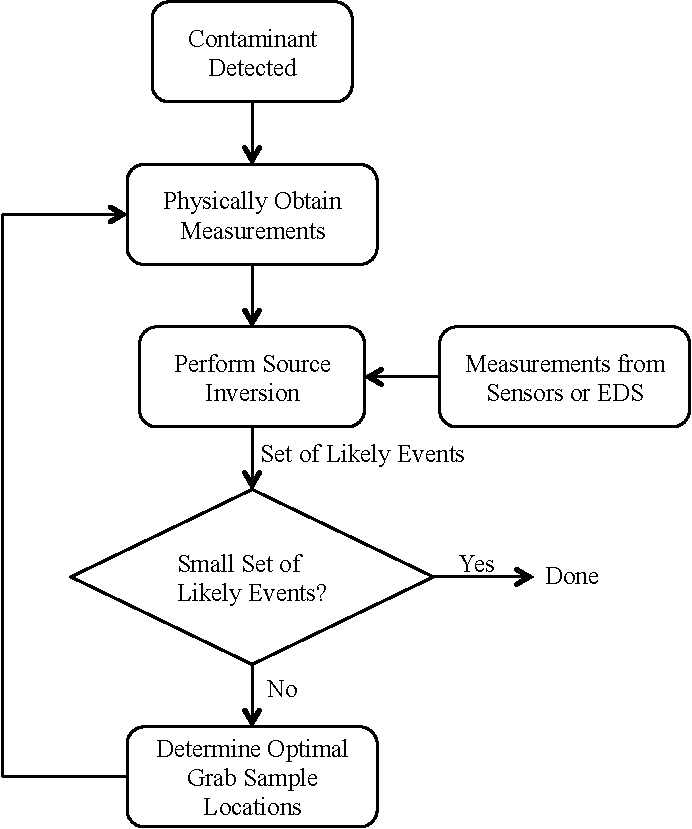
\includegraphics[scale=0.6]{graphics/inversion_strategy.pdf}
\caption{Illustration of the source inversion and grab sample cycling strategy.}
\label{fig:inversion_flowchart}
\end{center}
\end{figure}

\subsection{Case Study}
Since real system data is not available, the \code{measuregen}
executable is used to generate simulated data for the contamination incident in the following case study.  In this simulation, 
a conservative contaminant is injected into node 163 of EPANET
Example Network 3 (Net3) starting at 8 AM.  The Bayesian probability
based formulation [\ref{sec.bayesian_algorithm}] is used in
the \code{inversion} subcommand to identify the possible contamination
sources. Figure \ref{fig:case_study_setup} shows the fixed sensor
locations in blue while the original contamination location is shown
in red.  The CWS consists of five fixed sensors that provide
measurements every 15 minutes (set as a command line option in \code{measuregen}).

\begin{figure}[ht!]
\begin{center}
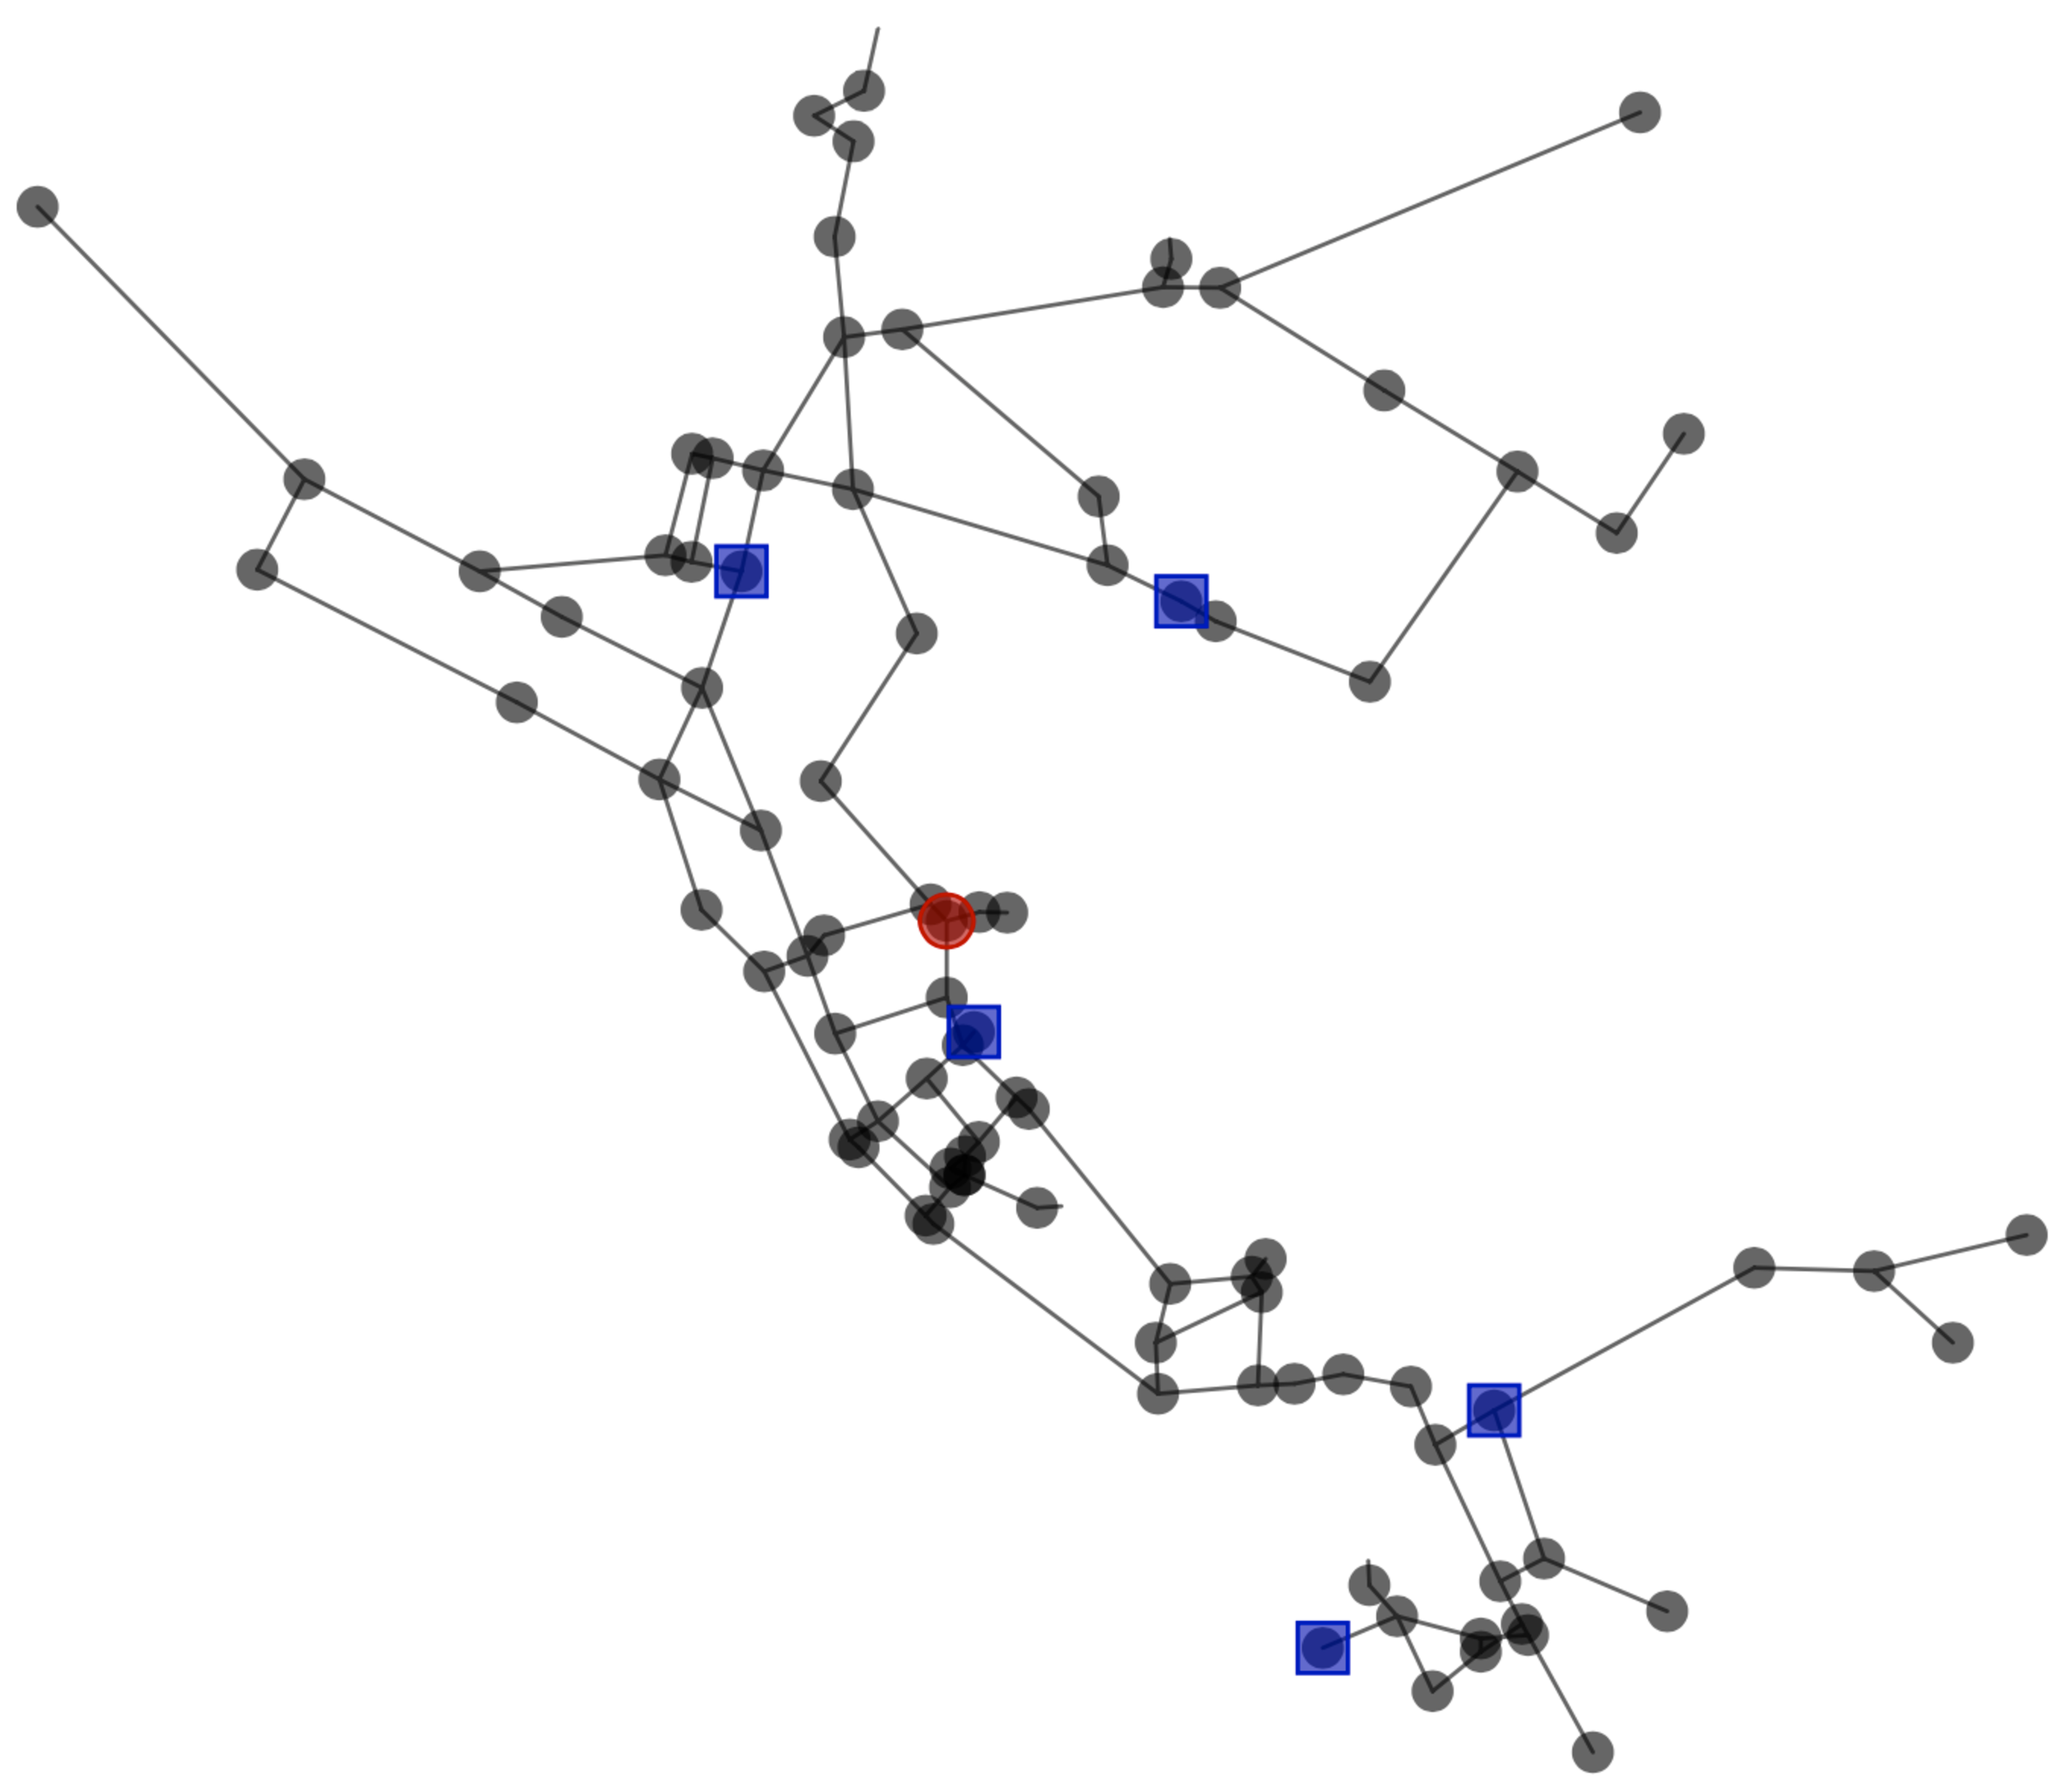
\includegraphics[scale=0.25]{graphics/inversion_cs_setup.pdf}
\caption{Fixed sensors (blue) and contamination location (red) for case study.}
\label{fig:case_study_setup}
\end{center}
\end{figure}

All the files required for this case study are provided in the \code{examples/case\_studies/inversion} folder.
  
The case study is a composed of three cycles of source inversion and grab sampling to reduce the number of possible contamination source 
locations. During each cycle, the \code{inversion} subcommand uses the following data:
\begin{itemize}
\item Net3.inp - EPANET Example Network 3 input (INP) file.
\item MEASURES.dat - Measurements file binary (yes/no) results from fixed sensors and grab samples (generated using \code{measuregen} executable).
\item \textit{<output\_prefix>}\_Likely\_Nodes.dat - Likely nodes file containing a list of feasible nodes to consider as possible contamination source nodes. 
This file is only used in cycles 2 \& 3. 
\end{itemize}      
The \code{inversion} subcommand outputs a YAML file with a list of possible contamination sources. 
A TSG file is also created that provides information about the possible contamination incidents. This file 
can be used in the \code{grabsample} subcommand. Thereafter, Cycles 1 \& 2 use the following data to determine optimal sample location:

\begin{itemize}
\item Net3.inp - EPANET Example Network 3 input (INP) file.
\item \textit{<output\_prefix>}\_profile.tsg - TSG file which contains a list of likely injections obtained 
from the \code{inversion} subcommand from the preceding cycle.
\item Sample time - Time in the future when the samples are expected to be taken. This is generally the current time 
plus the time it would take the sample teams to obtain measurements. 
\item fixed\_sensors.dat - List of fixed continuous sensor locations. This is used to avoid fixed sensors being selected
as grab sample locations.  

\end{itemize}

\subsection{Cycle 1}
At 8:15 AM, the sensor located at node 167 detects abnormal water quality. Further confirmation is made with another positive 
measurement at 8:30 AM. At this point, the measurement data from the past 8 hours is used to perform source inversion. 
The \code{inversion} subcommand identifies 24 possible injection locations as shown in red 
in Figure \ref{fig:case_study_cycle1}. The \code{grabsample} subcommand is then used to identify additional measurement 
locations that will reduce the number of possible injection locations. 
The utility has three teams available to gather manual grab samples and it takes 30 minutes for each team to 
obtain the manual samples. The \code{grabsample} subcommand identifies the three optimal grab sample locations 
shown in blue and the possible injection nodes in red in Figure \ref{fig:case_study_cycle1}.             

\begin{figure}[!ht]
\begin{center}
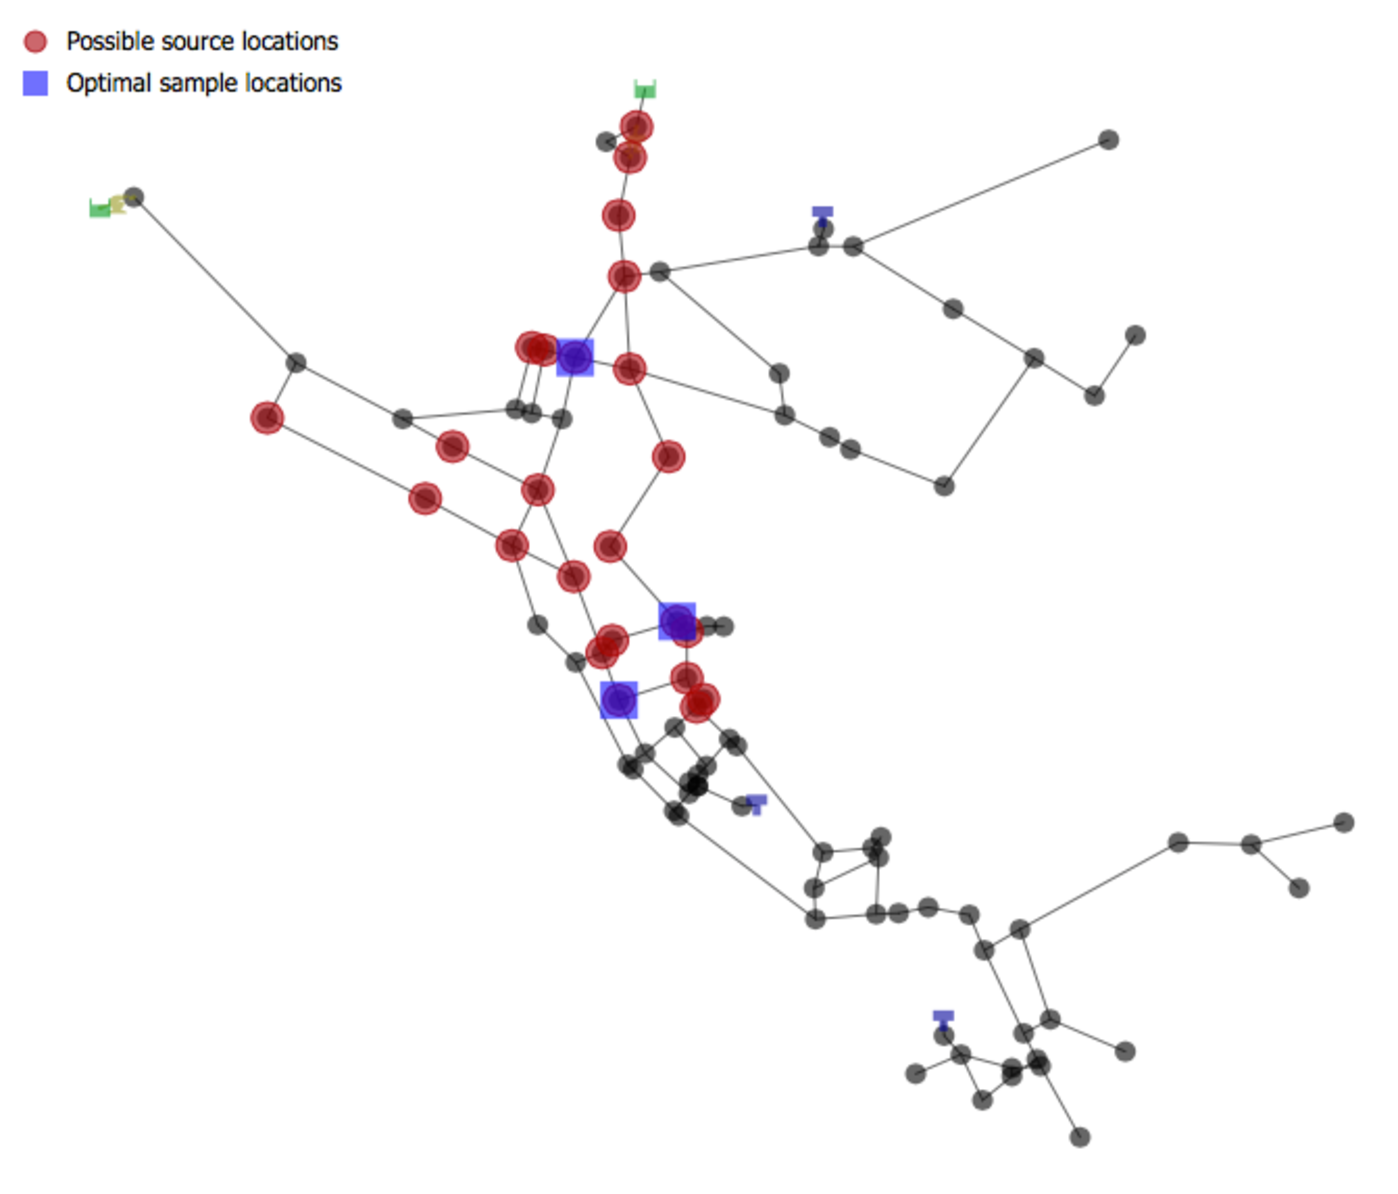
\includegraphics[scale=0.6]{graphics/inversion_cs_cycle1.pdf}
\caption{Cycle 1 identified optimal grab sample locations (blue).}
\label{fig:case_study_cycle1}
\end{center}
\end{figure}

The files required and generated during this cycle of source inversion and grab sample 
are provided in the \code{examples/case\_studies/inversion/Cycle1} folder. 

\subsection{Cycle 2}
In the 30 minutes that the sampling teams take to get manual grab sample measurements from the locations identified in Cycle 1, 
new measurements are also available from the fixed sensors in the CWS. It is assumed that
the sampling teams have field instruments that can provide them with a yes/no indication of the
presence or absence of a contaminant.  
At 9:00 AM, these new measurements are used to perform source inversion again. 
This time the \code{inversion} subcommand identifies seven possible injection locations as shown in Figure \ref{fig:case_study_cycle2}. 
In Cycle 2, the possible sources were restricted to the 24 nodes identified in Cycle 1 using the feasible nodes option. 
Again a 30-minute delay for sample collection and three sample teams were used in the \code{grabsample} subcommand to identify 
the optimal grab sample locations at 9:30 AM. These grab sample locations (blue) and 
the possible injection nodes (red) are shown in Figure \ref{fig:case_study_cycle2}.

\begin{figure}[!ht]
\begin{center}
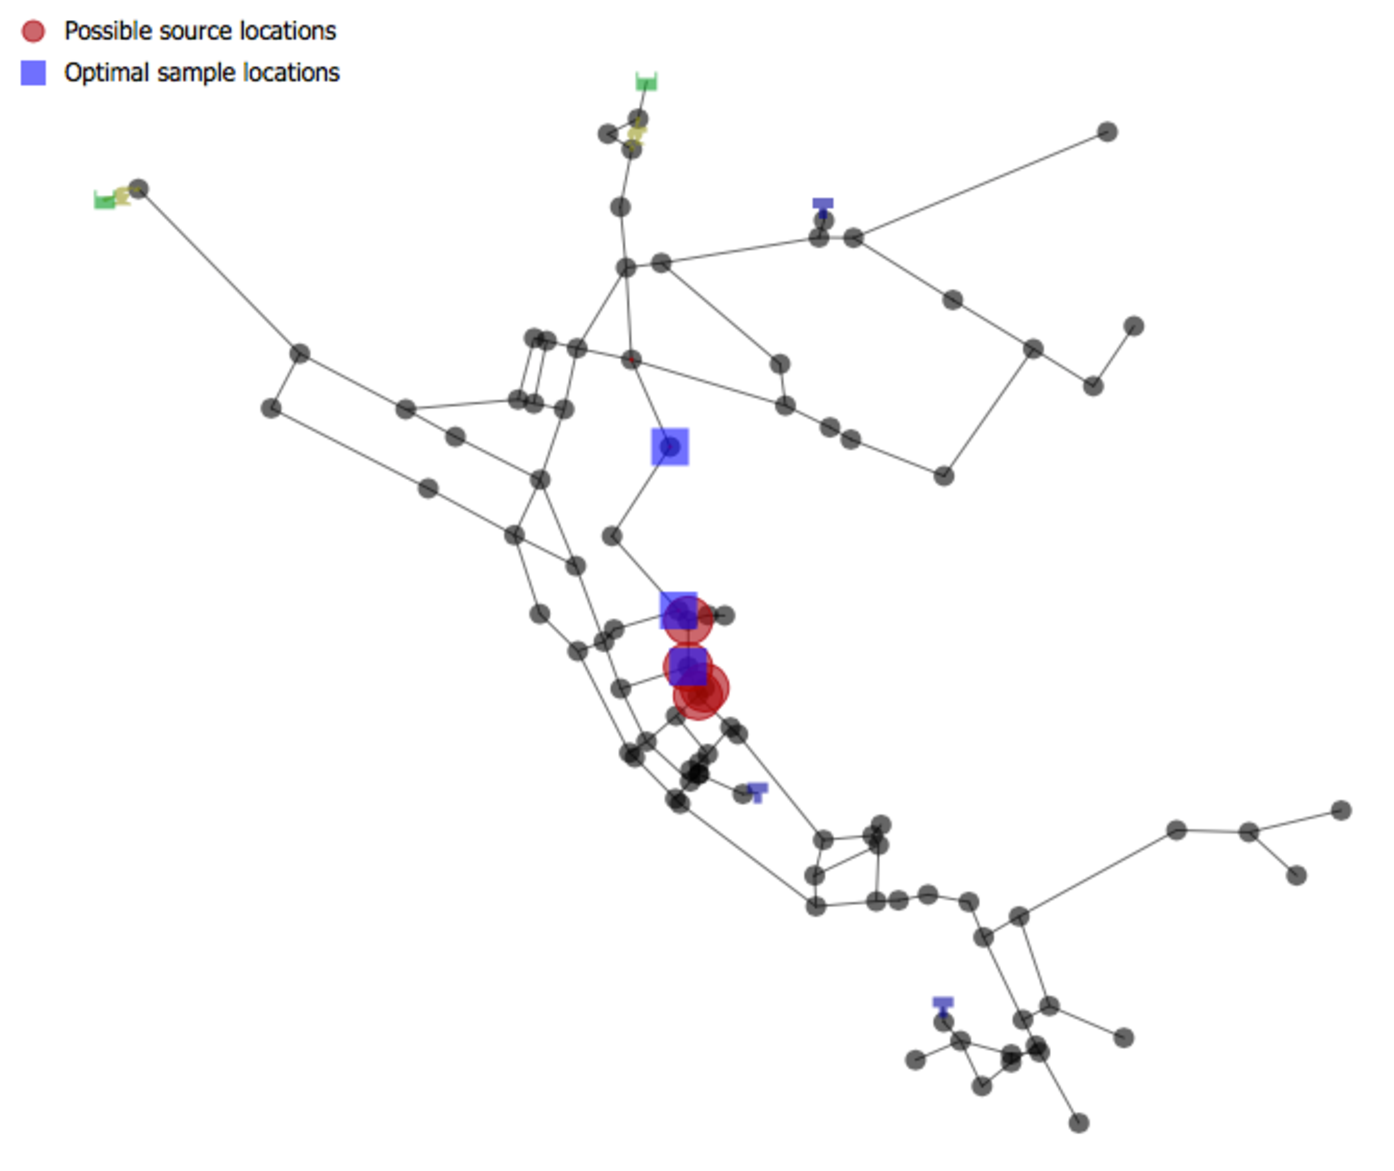
\includegraphics[scale=0.6]{graphics/inversion_cs_cycle2.pdf}
\caption{Cycle 2 identified optimal grab sample locations (blue).}
\label{fig:case_study_cycle2}
\end{center}
\end{figure}

The files required and generated during this cycle of source inversion and grab sample are 
provided in the \code{examples/case\_studies/inversion/Cycle2} folder.  
        
\subsection{Cycle 3}
Grab sample measurements are obtained at 9:30 AM from the optimal locations identified in Cycle 2. 
These along with the new measurements obtained from the fixed sensors are used to perform source inversion again. 
Only the seven possible injection nodes obtained in Cycle 2 are considered as feasible nodes in the \code{inversion} subcommand 
for Cycle 3. Three possible injection locations as shown in Figure \ref{fig:case_study_cycle3} are identified in this cycle.

\begin{figure}[!ht]
\begin{center}
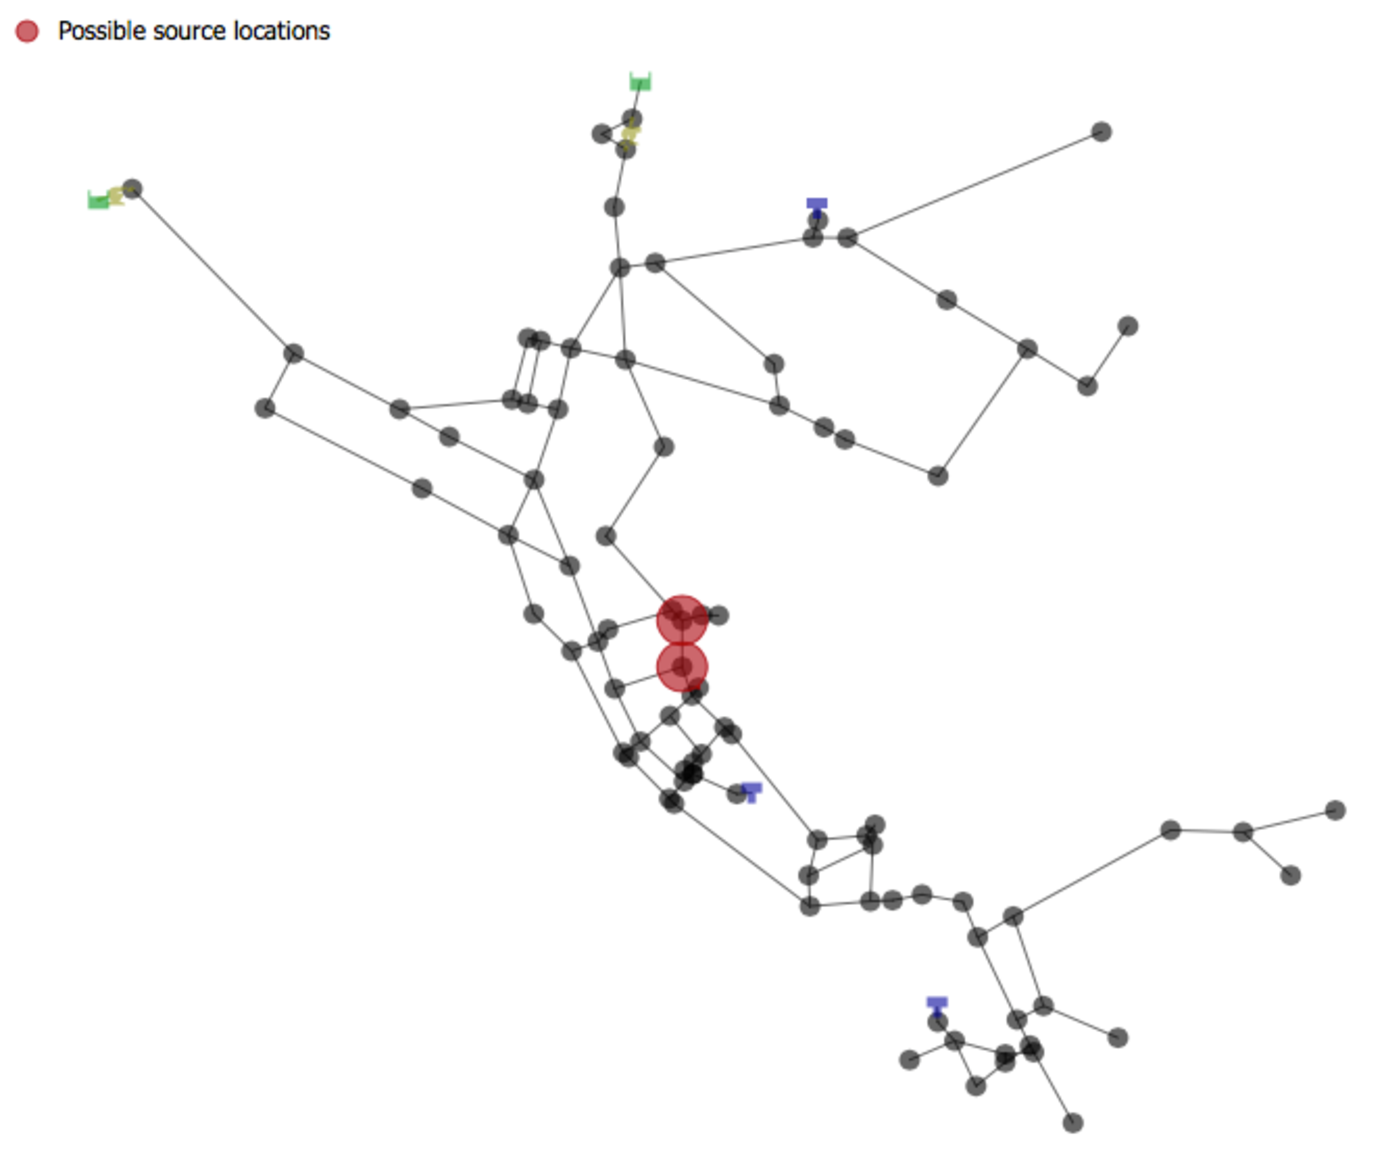
\includegraphics[scale=0.6]{graphics/inversion_cs_cycle3.pdf}
\caption{The possible injection nodes (red) identified in Cycle 3.}
\label{fig:case_study_cycle3}
\end{center}
\end{figure}

Since the water utility has three sampling teams available, the teams can directly inspect the three possible injection locations 
identified in this cycle to confirm the true injection location.  

\newpage

\section{Uncertainty Reduction with Grab Samples Case Study}\label{chap:samplingCase} 
\label{sampling_case_study}
The following case study illustrates how the functionality of the \code{inversion}, \code{grabsample} and \code{uq} subcommands 
can be used in tandem to identify multiple sampling cycles that reduce uncertainty in the extent of contamination.
The approach uses successive measurements obtained from manual grab samples to find the contamination plume.  
Figure \ref{fig:ureduction_flowchart} illustrates the methodology.
A contamination incident is first suspected following a customer inquiry or detection from a fixed continuous 
sensor in the Contamination Warning System (CWS). 
At this stage, a team is sent out to gather manual grab samples at and around the location of first detection. 
Discrete yes/no measurements from these manual grab samples along with the measurement from contamination warning system 
are then used to estimate the probability that nodes in the network are contaminated.
The probability of node contamination provides a metric of uncertainty quantification. Given a particular confidence level (e.g., 95\%), 
nodes can be categorized according to their probability of contamination: LY for ``likely yes,'' LN for ``likely no'' and UN for ``unknown.''  

If a sufficiently small number of nodes remain uncertain, then the process is terminated, otherwise further sampling cycles are required. 
This cycle of collecting manual grab samples is continued until the contamination plume is estimated with a good level of confidence. 
\begin{figure}[!ht]
\begin{center}
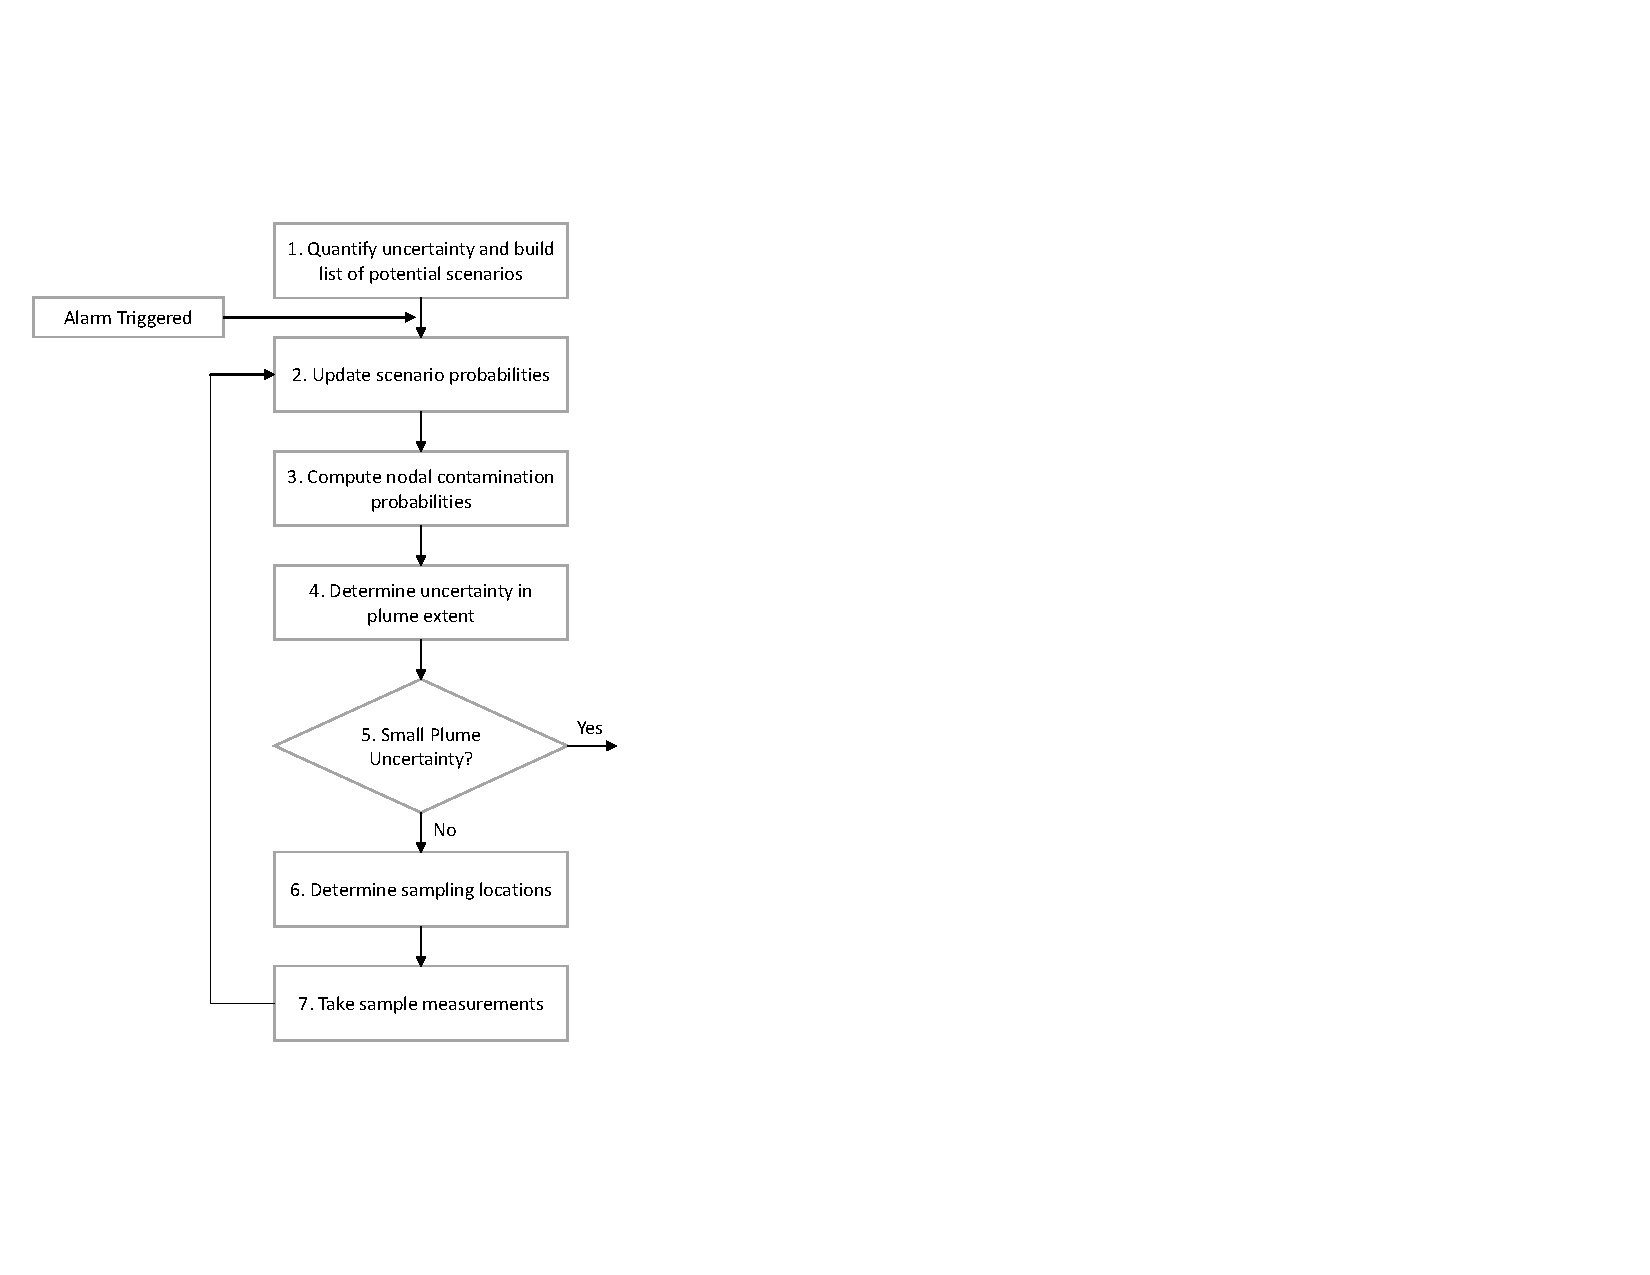
\includegraphics[scale=0.6]{graphics/uncertaintyprocess3.pdf}
\caption{Illustration of the source inversion and grab sample cycling strategy.}
\label{fig:ureduction_flowchart}
\end{center}
\end{figure}

\subsection{Case Study}
Since real system data is not available, the \code{measuregen}
executable is used again to generate simulated data for a contamination incident in the following case study.  In this simulation, 
a conservative contaminant is injected into node 115 of EPANET
Example Network 3 (Net3) at 8 am.  The set of potential scenarios includes 10 hydraulic realizations with 97 different injection locations. All of the files required 
for this case study are provided in the \code{examples/case\_studies/sampling} folder.
  
The case study is composed of four sampling cycles to reduce uncertainty in the extent of contamination. The initial warning is 
raised at 10 am. From this time, the procedure in Figure \ref{fig:ureduction_flowchart} is followed to reduce uncertainty by gathering 
grab samples every hour. In each sampling cycle, three additional samples are collected. Given the information provided by the new samples, 
the probability distribution of scenarios is updated following Bayesian statistics. Then, the methodology proposed in Section \ref{uqn_algorithms} 
is followed to quantify uncertainty. To facilitate the analysis, a script was implemented in Python to run the sampling cycles in a loop, which is the signals.py file provided in the \code{examples/case\_studies/sampling/cycling} folder. 
The execution of the script follows the same convention as the WST subcommands:

\begin{unknownListing}
python wst/packages/pywst/pywst/cycling/signals.py cycle <configfile>
\end{unknownListing}

The options for the script are the same as the options provided in the sections of the \code{inversion}, \code{uq} and \code{grabsample} subcommands. 
Some additional options to specify duration of each cycle and number of cycles are added. The configuration file for this case study, sampling\_case\_study.yml, 
is shown in Figure \ref{fig:case_study_conf}.  

\begin{figure}[!ht]
  \unknownInputListing{../../examples/case_studies/sampling/sampling_case_study.yml }{}{1}{13}
  \caption{The configuration file for sampling case study.}
  \label{fig:case_study_conf}
\end{figure}

\subsection{Cycle 0}
At 10 AM, the contamination warning system detects abnormal water quality at nodes 40 and 111. The measurement data from those two locations is used to 
perform a Bayesian update in the probability of scenarios. At this point, given the probability distribution of scenarios, 73 possible scenarios are 
identified as most likely. The uncertainty in the number of scenarios is evident in the uncertainty quantification as most of the nodes are deemed unknown (UN). 
Figure \ref{fig:case_study_cycle1} shows in yellow all locations that are considered uncertain to have contamination. 
The utility has three teams available to gather manual grab samples and it takes 60 minutes for each team to 
obtain the manual samples. The probability-based formulation in Chapter \ref{chap:grabsample} identifies the three optimal grab sample locations shown 
in dark gray/black in Figure \ref{fig:case_study_cycle1}.             

\subsection{Cycle 1}
At 11:00 AM, the new measurements are used to perform a Bayesian update and an uncertainty quantification. 
This time the number of uncertain nodes is reduced by half as shown in Figure \ref{fig:case_study_cycle2}. Nodes in red are likely to be contaminated (LY) and 
nodes in blue are likely to not be contaminated (LN). Again a 60-minute delay for sample collection and three sample teams were used in the probability-based 
formulation in Chapter \ref{chap:grabsample} to identify the optimal grab sample locations at 12:00 PM. The three new and three previous grab sample locations (dark gray/black) are shown in Figure \ref{fig:case_study_cycle2}.
        
\subsection{Cycle 2}
Grab sample measurements are obtained at 12:00 PM from the optimal locations identified in second cycle of the \code{grabsample} subcommand. 
These are used to perform Bayesian update and an uncertainty quantification again. 
Only seven nodes remain uncertain (UN) as to whether they are contaminated in this cycle. As the uncertainty is still not small enough, three more sampling locations are 
identified by solving the probability based formulation of Chapter \ref{chap:grabsample}. The three new grab sample locations plus the six previous (dark gray/black) are shown in 
Figure \ref{fig:case_study_cycle3}.

\subsection{Cycle 3}
Grab sample measurements are obtained at 1:00 PM from the optimal locations identified in in third cycle of the \code{grabsample} subcommand. 
With this new information, the Bayesian update and the uncertainty quantification lead to zero nodes classified as uncertain (all are likely yes or likely no). The three new grab sample locations plus the nine previous (dark gray/black) are shown in Figure \ref{fig:case_study_cycle4}. Only 11 grab sample locations are shown in this cycle since one of the locations was selected to be sampled twice, since different sampling times can provide different measurement data. 

\begin{figure}[!h]
\centering
\begin{subfigure}{0.49\textwidth}
\centering
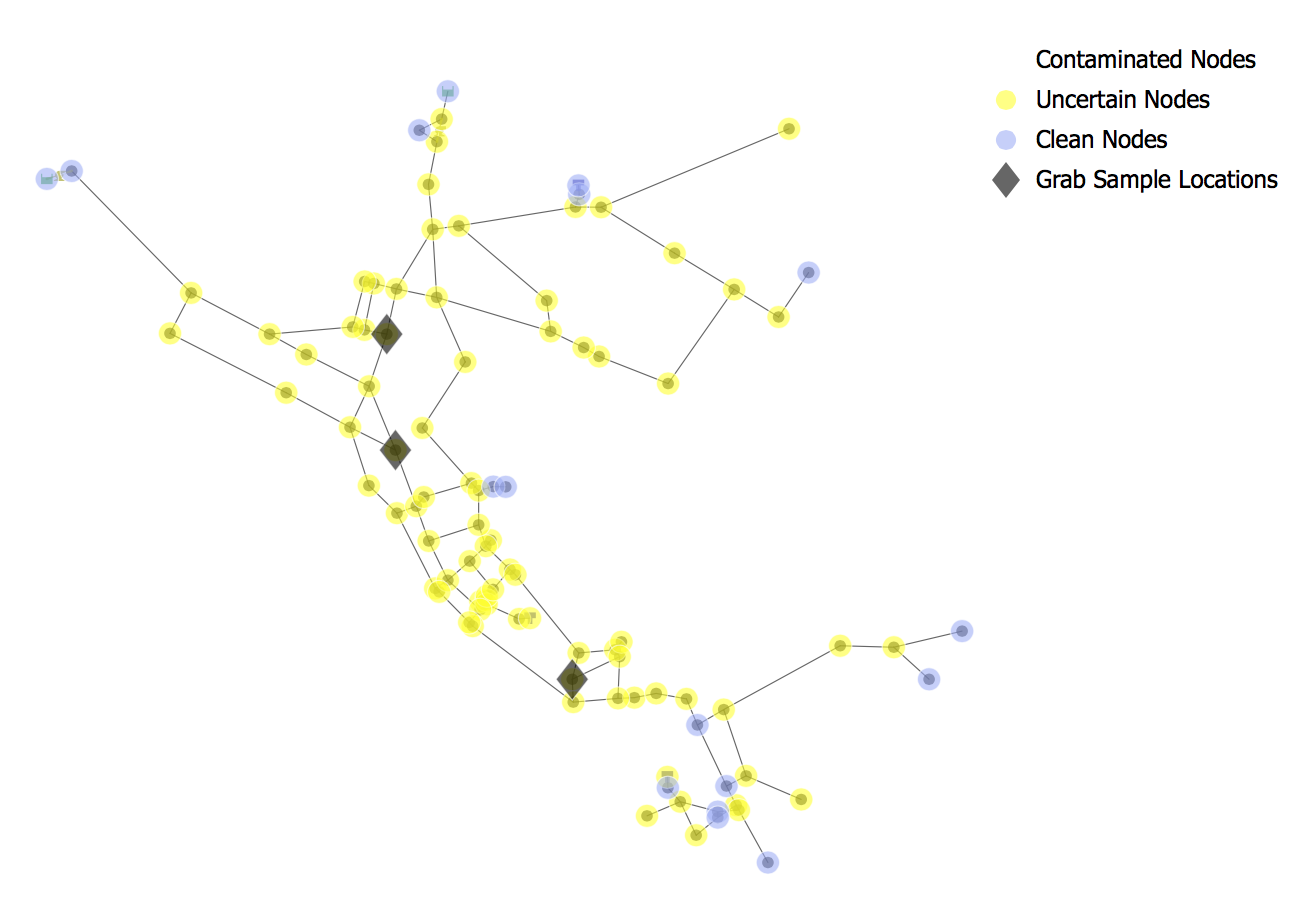
\includegraphics[width = \textwidth]{graphics/sampling_cs_cycle1.png}
\caption{Cycle 0}
\label{fig:case_study_cycle1}
\end{subfigure}
\begin{subfigure}{0.49\textwidth}
\centering
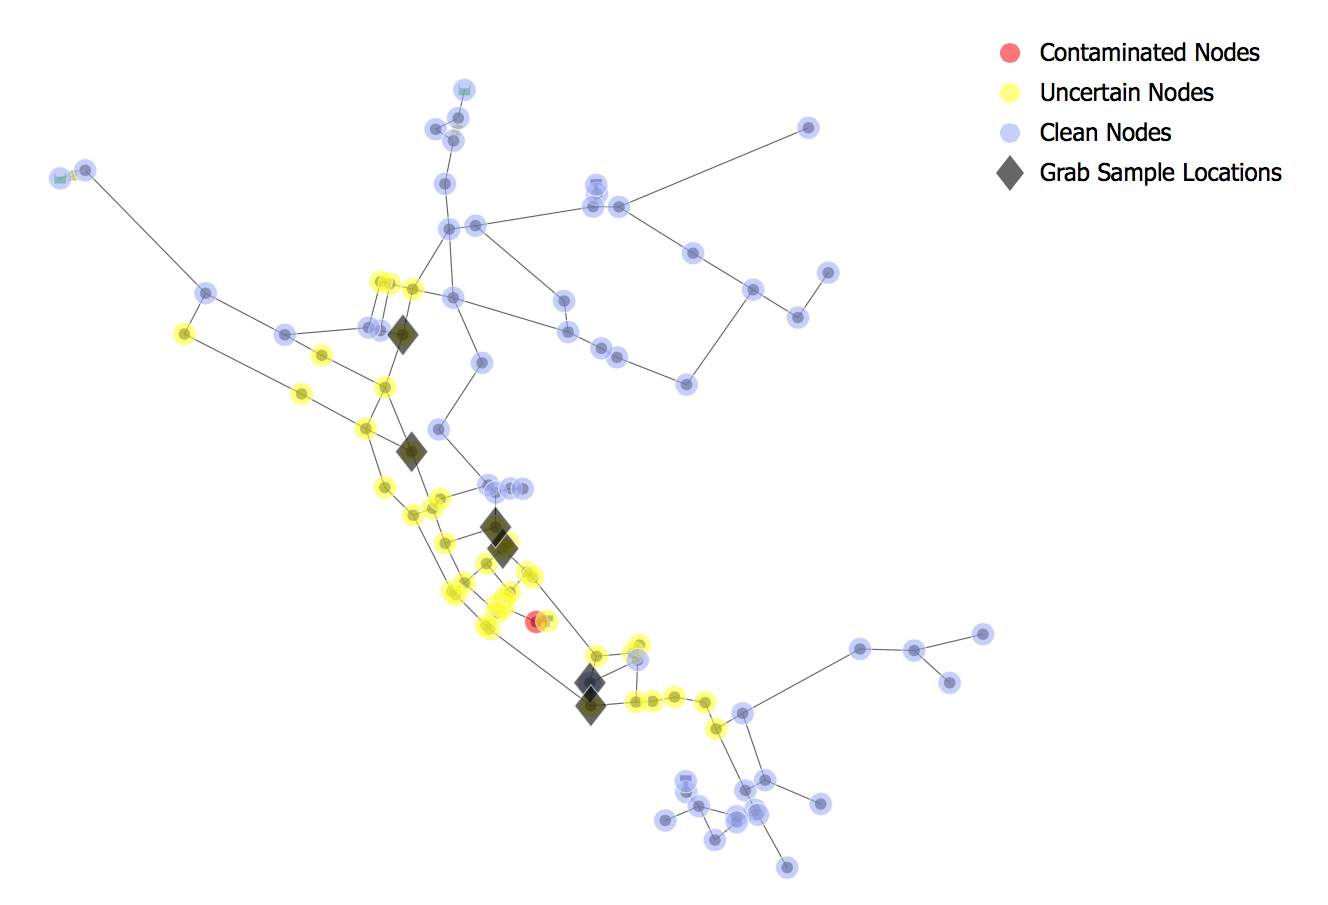
\includegraphics[width = \textwidth]{graphics/sampling_cs_cycle2.png}
\caption{Cycle 1}
\label{fig:case_study_cycle2}
\end{subfigure}
\centering
\begin{subfigure}{0.49\textwidth}
\centering
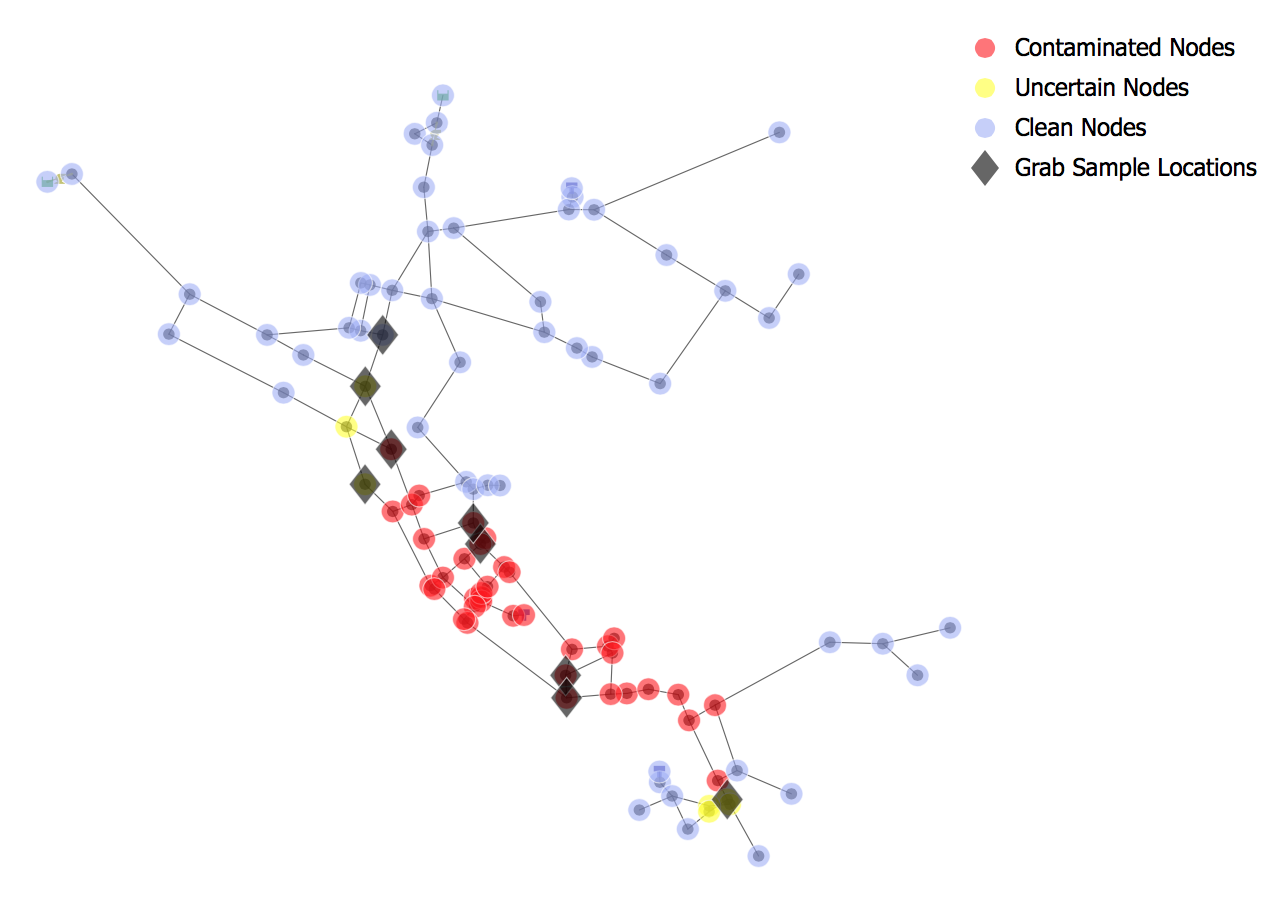
\includegraphics[width = \textwidth]{graphics/sampling_cs_cycle3.png}
\caption{Cycle 2}
\label{fig:case_study_cycle3}
\end{subfigure}
\begin{subfigure}{0.49\textwidth}
\centering
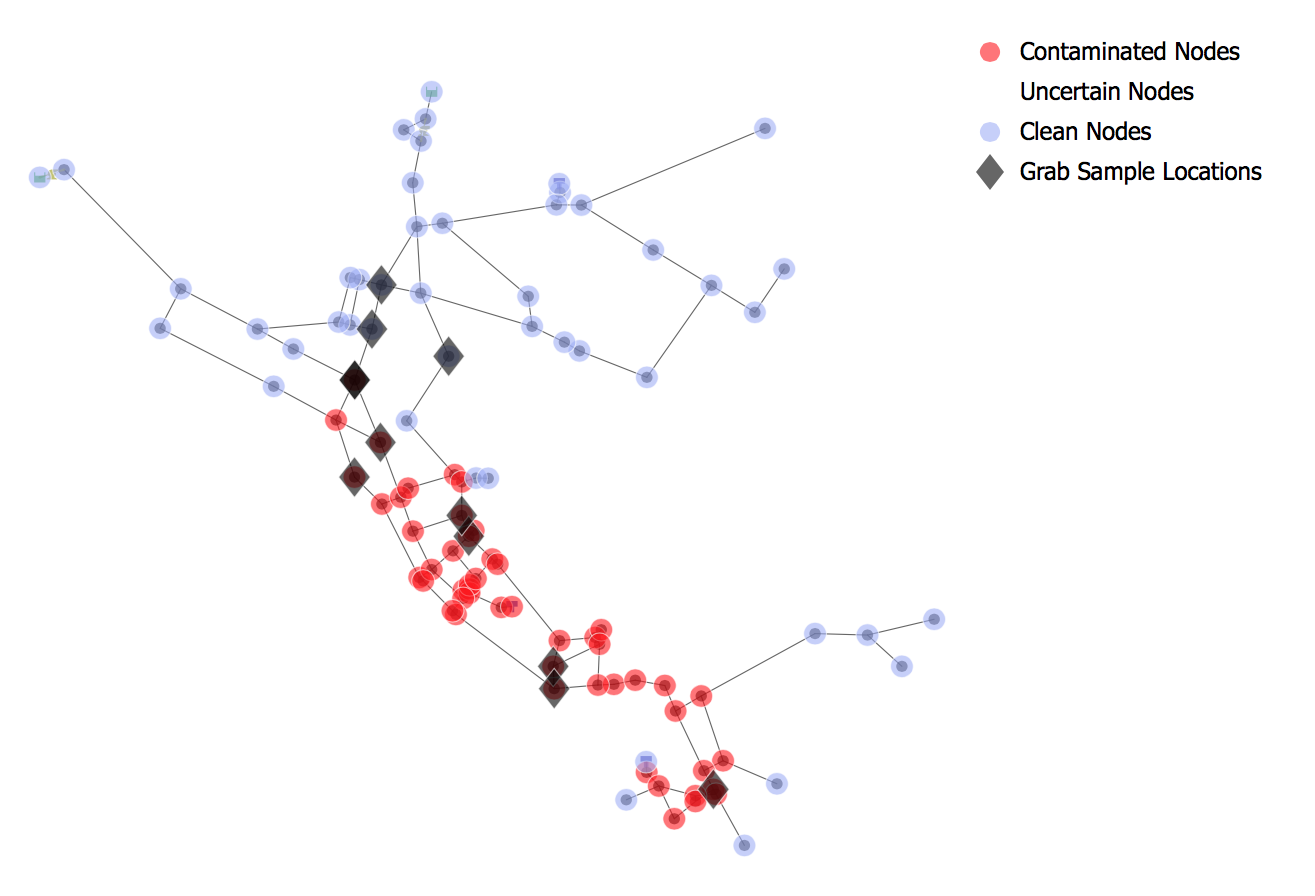
\includegraphics[width = \textwidth]{graphics/sampling_cs_cycle4.png}
\caption{Cycle 3}
\label{fig:case_study_cycle4}
\end{subfigure}
\caption{EPANET Example Network 3 with grab sample locations (dark gray/black diamonds), contaminated nodes (red circles), uncertain nodes (yellow circles), and clean nodes (blue-gray circles) identified for each of the cycles in the case study.}
\label{fig:gs_uq_case_study}
\end{figure}

\newpage

\newpage
\section{Flushing with Source Identification Case Study}\label{chap:flushCase} 
\label{flushing_case_study}
When a water utility becomes aware of a water quality issue either through 
customer complaints or water quality sensor alarms, they often open a hydrant to 
flush a portion of the distribution network in order to bring new water into the 
area and increase the chlorine residual. This case study examines how WST can 
be used to identify effective flushing locations following a water quality 
sensor alarm using the the \code{flushing}, \code{inversion} and 
\code{grabsample} subcommands. All files required to run the case study 
are provided in the \code{examples/case\_studies/flushing} folder.

The EPANET input file for this example is Net6.inp, which has a simulation duration 
of seven (7) days starting at midnight. The network is assumed to include a contamination 
warning system (CWS) with ten optimally placed water quality sensors and an 
event detection system in operation. The 10 sensors are located at 
JUNCTION-1617, JUNCTION-199, JUNCTION-2297, 
JUNCTION-2716, JUNCTION-2930, JUNCTION-3023, JUNCTION-435, JUNCTION-552, 
JUNCTION-675 and JUNCTION-831. The sensors were optimally placed 
using the \code{sp} subcommand. 
Figure \ref{fig:wds_sensors} shows the water distribution network and the location of the 
water quality sensors. The CWS provides binary values every 15 minutes from each sensor 
location. The binary value is zero if water quality conditions 
are normal or one if the conditions are abnormal.  

\begin{figure}[h!]
\begin{center}
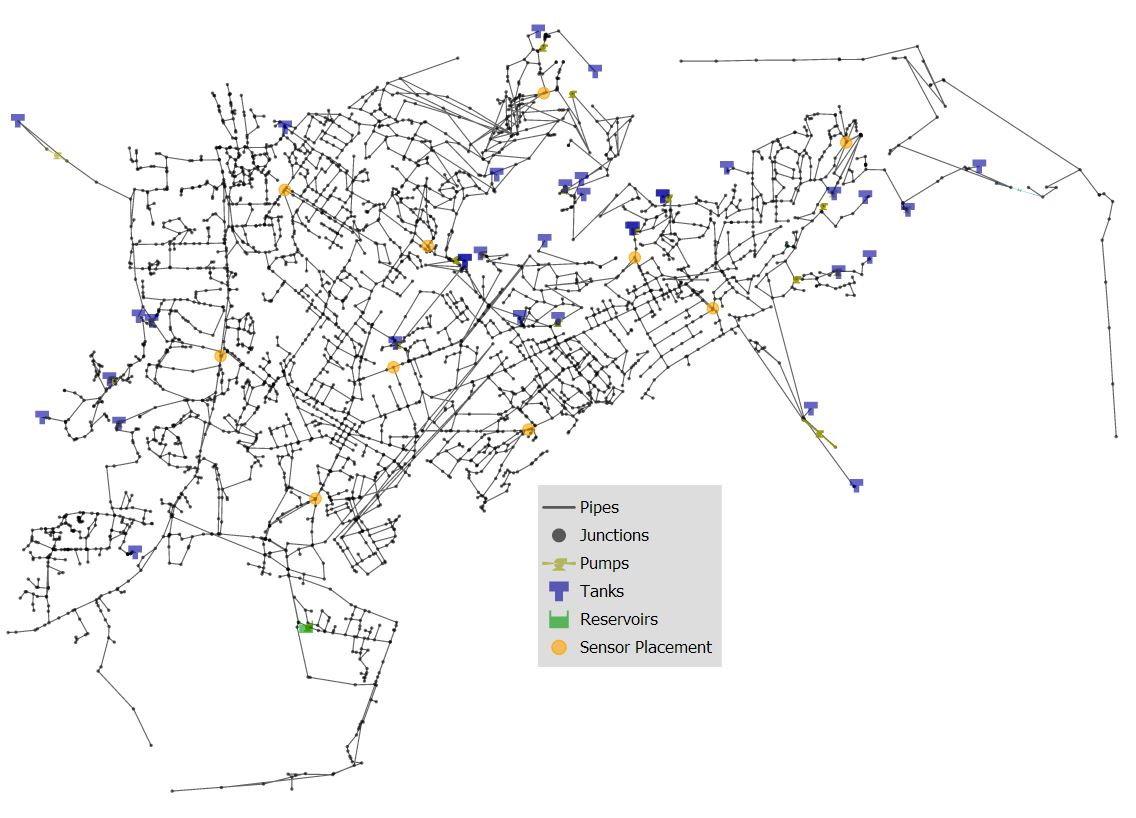
\includegraphics[scale=0.6]{graphics/Net6_Sensors.JPG}
\caption{Net6 water distribution network with water quality sensors.}
\label{fig:wds_sensors}
\end{center}
\end{figure}
 
At 10:15 AM, the CWS alerts water utility staff to abnormal water quality occurring 
at water quality sensor located at JUNCTION-1617 in water distribution network model. 
Figure \ref{fig:wds_sensors_detect} shows the JUNCTION-1617 highlighted as the sensor 
location with a positive detection of contamination in the network.  

\begin{figure}[h!]
\begin{center}
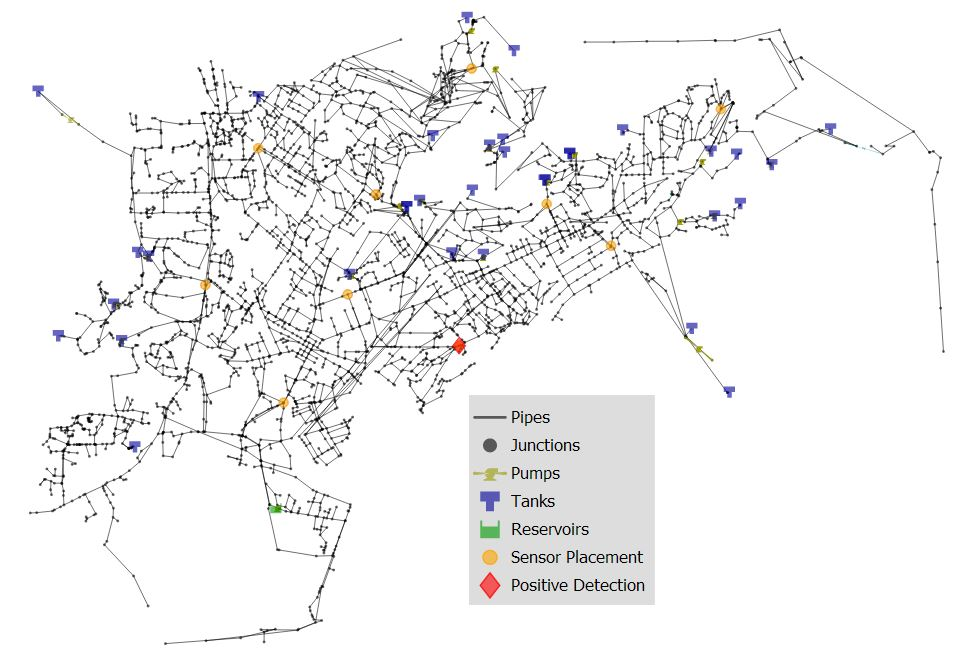
\includegraphics[scale=0.6]{graphics/Net6_Sensors_detect.JPG}
\caption{Net6 with positive contamination detection at JUNCTION-1617.}
\label{fig:wds_sensors_detect}
\end{center}
\end{figure}

The water utility must now decide how to proceed. The staff checks their 
consequence management plan and sends out a team to ensure that the water quality 
sensor is working properly. The water utility staff determines 
that a contamination incident is possible and they would like to identify the source.  
Source identification allows the water utility to determine the extent of contamination (or spread) and possibly
shut off any continuing injection of contaminants.  
Using the CWS information from the past 35 hours, provided in the measurements file 
Net6\_CWS\_MEASURES.dat, and the Net6 INP file, the \code{inversion} subcommand is used to 
identify the possible sources of the contamination. The inversion configuration file, 
Net6\_inversion.yml, and the measurements file are provided in the \code{examples/case\_studies/flushing} folder.

The \code{inversion} subcommand can be executed using the following command line:

\begin{unknownListing}
wst inversion Net6_inversion.yml
\end{unknownListing}  

Figure \ref{fig:wds_sources} shows the 25 possible contamination sources identified by the 
\code{inversion} subcommand.  

\begin{figure}[h!]
\begin{center}
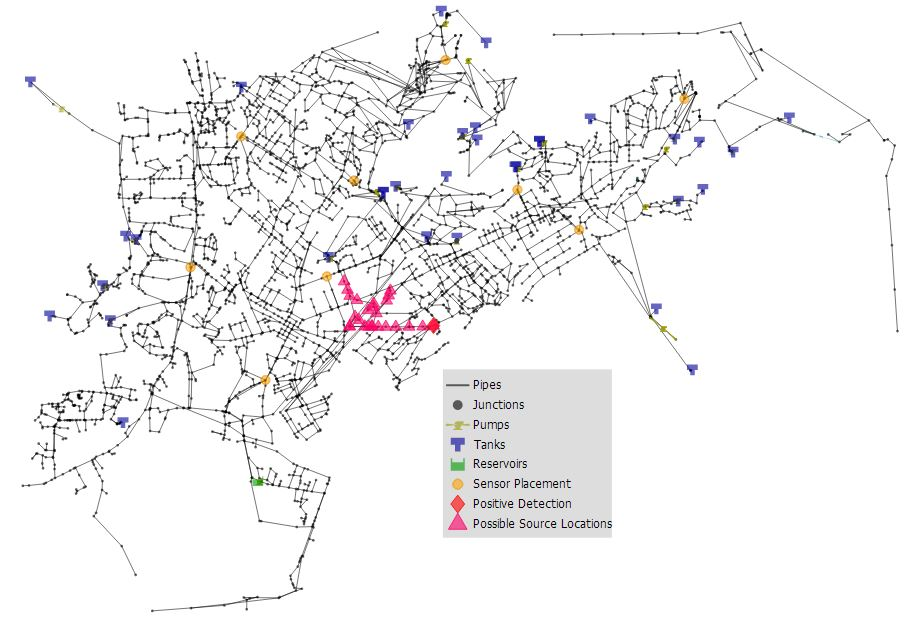
\includegraphics[scale=0.6]{graphics/Net6_possible_sources.JPG}
\caption{Net6 with possible contamination sources identified by \code{inversion} subcommand.}
\label{fig:wds_sources}
\end{center}
\end{figure}

Since flushing is a common response to abnormal water quality, the water utility staff decide 
to open hydrants to flush the contaminated water out of the network. To determine the most 
effective flushing locations, the staff simulates contamination incidents from each 
possible contamination source location using the TSG file produced from the \code{inversion} subcommand. 
From these simulations, the possible extent of contamination from each source location is identified. 
The nodes in the water distribution network model which are calculated to have 
contaminant concentrations above zero at the starting of flushing (12:00 PM, 
approximately two hours after detection) are considered as the initial starting points for the network 
solver option in the \code{flushing} subcommand. These initial starting points 
are the first node locations that are going to be evaluated in terms of the impact metric  
and then as the process continues, the solver will look at all of the nodes that are 
connected to these initial points to determine their impact metrics. Figure \ref{fig:wds_impacted_nodes} 
shows the nodes impacted by the 25 possible contamination source locations.  

\begin{figure}[h!]
\begin{center}
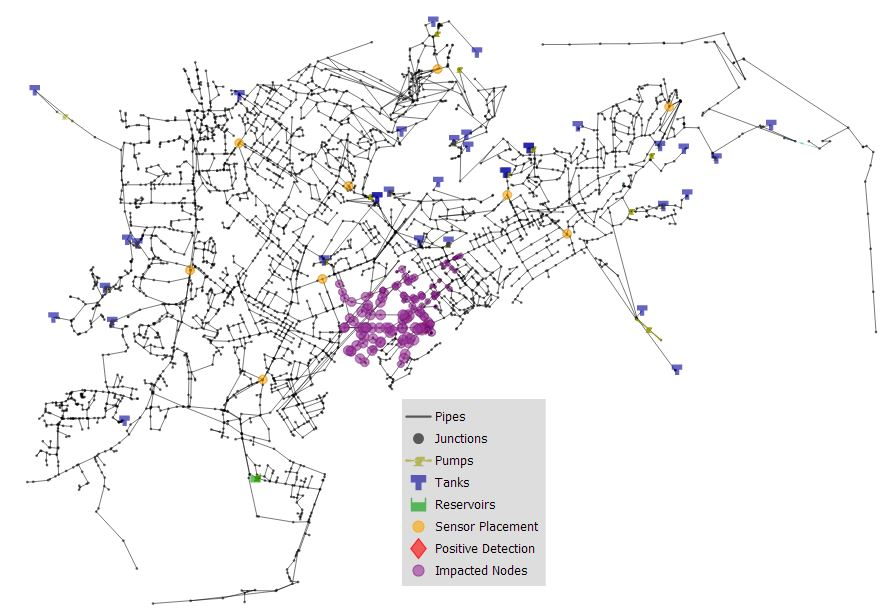
\includegraphics[scale=0.6]{graphics/Net6_imapcted_nodes_25inj.JPG}
\caption{Net6 with nodes impacted by the 25 possible contamination sources.}
\label{fig:wds_impacted_nodes}
\end{center}
\end{figure}

The water utility decides to open two hydrants to flush the contaminated water out of the network, 
since the extent of contamination for the possible 25 contamination sources (as seen in 
Figure \ref{fig:wds_impacted_nodes}) is not very large at the 
start of flushing at 12:00 PM. To identify effective 
flushing locations, the \code{flushing} subcommand is used. This command requires the following 
files as specified in the flushing configuration file, Net6\_flush\_2nodes.yml:

\begin{itemize}
\item Net6.inp - Net6 EPANET input (INP) file.
\item Net6\_inv1\_profile.tsg - The TSG file created by the \code{inversion} subcommand.
\item Net6\_bio.tai - The TAI file describing the dose-response characteristics for the assumed contaminant. 
This file is required when using the population exposed (PE) impact metric. 
\end{itemize}  

In addition, characteristics of the flushing response are also defined in the 
flushing configuration file. These include:

\begin{itemize}
\item A list of nodes that can be flushed - All non-zero demand (NZD) nodes 
\item The maximum number of nodes which can be flushed simultaneously - 2 
\item The flushing rate - 1100 gallons/min
\item The flushing duration - 8 hours 
\item The response time delay (time between detection and start of flushing) - 1 hour
\end{itemize}  

Other information provided in the flushing configuration file include the 
impact metric that is going to be minimized (PE), the nodes where water 
quality sensors are located, the type of solver (network solver), 
and the initial starting points for the network solver (JUNCTION-1881 and 
JUNCTION-1878). 

The \code{flushing} subcommand can be executed using the following command line:

\begin{unknownListing}
wst flushing Net6_flush_2nodes.yml
\end{unknownListing}  

Figure \ref{fig:wds_flushing_nodes} shows the flushing nodes identified by 
the \code{flushing} subcommand. The flushing nodes identified are JUNCTION-1881 
and JUNCTION-2233.  

\begin{figure}[h!]
\begin{center}
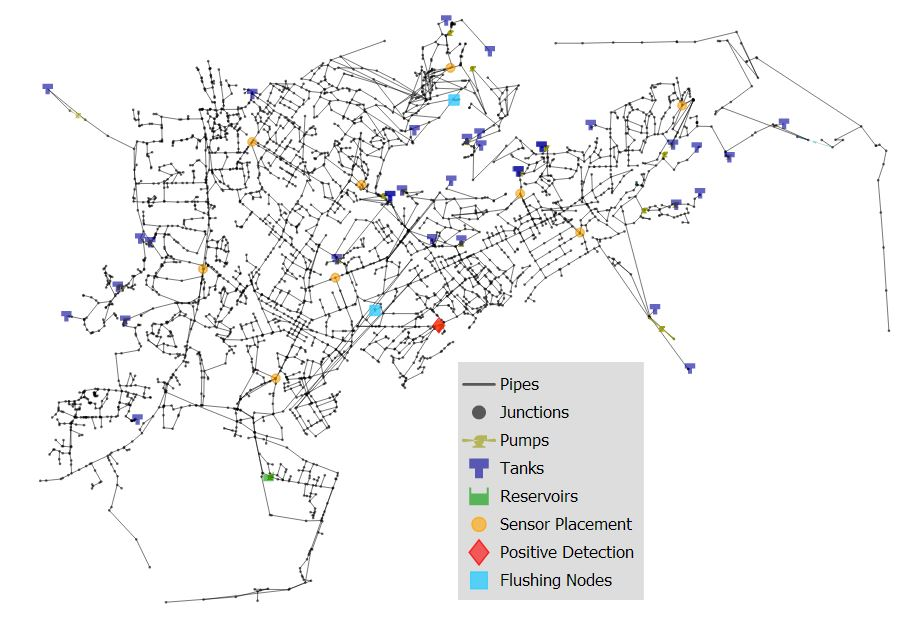
\includegraphics[scale=0.6]{graphics/Net6_2nodes_flushing.JPG}
\caption{Net6 with the flushing nodes identified by the \code{flushing} subcommand.}
\label{fig:wds_flushing_nodes}
\end{center}
\end{figure}

Since the identified flushing nodes were based upon the 25 possible contamination sources, 
the water utility staff evaluate the flushing response against each of the possible 
sources assuming it was the true source of the contamination. This option is available 
using EVALUATE as the type under the solver block of the flushing configuration file. An 
example flushing configuration file for the evaluate option is provided in 
Net6\_flush\_2nodes\_eval\_JUNC1617.yml in the \code{examples/case\_studies/flushing} folder. 
This example assumes that JUNCTION-1617 is the true source of contamination in the network 
and it evaluates the effectiveness of the identified flushing locations in terms of the 
PE metric. If JUNCTION-1617 is the true source, flushing at JUNCTION-1881 and JUNCTION-2233 
reduces the PE metric by only two percent (2\%).

% \todo{can you assume a different true source?  This one is among the worst.}

The \code{flushing} subcommand for this example can be executed using the following command line:

\begin{unknownListing}
wst flushing Net6_flush_2nodes_eval_JUNC1617.yml
\end{unknownListing}

Because the \code{inversion} subcommand solvers assume a continuous injection, the 
created TSG file has the contamination injection durations lasting as long as the 
simulation duration listed in the network INP file. Thus, the contamination injections 
start a little before the detection time and stop at the end of the simulation 
(seven days). Since an important response action would include shutting off the 
source of contamination, the TSG file is modified to stop the injection five 
hours after detection. Using the modified TSG file, the flushing response is evaluated 
against each of the 25 possible sources assuming it was the true source of the contamination.   
Figure \ref{fig:flushing_pe_reduction} shows the percent reduction in the PE metric 
for each of the 25 possible contamination sources with flushing alone (blue) and 
flushing with shutting off the contamination source (green). The percent 
reduction in the PE metric ranges from 24\% to 97\% for the flushing with source shut-off 
response action, which is an increase from the range of 2\% to 45\% for the flushing alone 
action. The highest percent reduction was if the true injection incident occurred at JUNCTION-1881.

\begin{figure}[h!]
\begin{center}
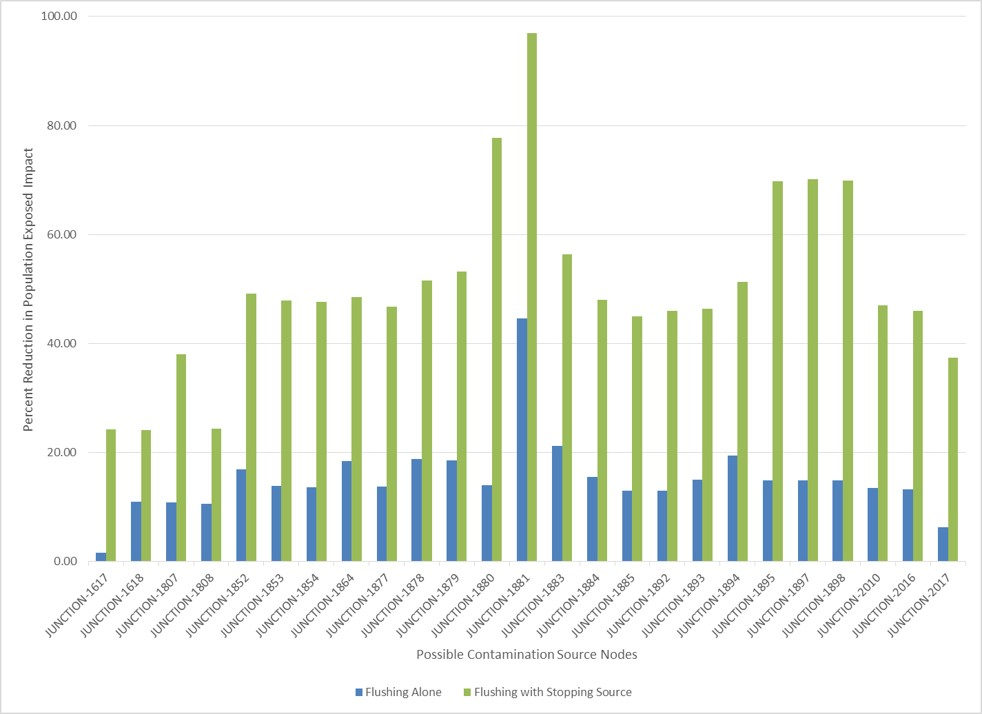
\includegraphics[scale=0.6]{graphics/flushing_pe_reduction.jpg}
\caption{The reduction in the PE metric for each of the 25 possible contamination sources.}
\label{fig:flushing_pe_reduction}
\end{center}
\end{figure}

% If the water utility wants to reduce the number of possible contamination sources 
% and improve the effectiveness of the flushing response, they could send staff to 
% manually collect grab samples to supplement the CWS measurements. 
 
% \todo{was grabsample used?}

\newpage
